\documentclass[ignorenonframetext,]{beamer}
\setbeamertemplate{caption}[numbered]
\setbeamertemplate{caption label separator}{: }
\setbeamercolor{caption name}{fg=normal text.fg}
\beamertemplatenavigationsymbolsempty
\usepackage{lmodern}
\usepackage{amssymb,amsmath}
\usepackage{ifxetex,ifluatex}
\usepackage{fixltx2e} % provides \textsubscript
\ifnum 0\ifxetex 1\fi\ifluatex 1\fi=0 % if pdftex
  \usepackage[T1]{fontenc}
  \usepackage[utf8]{inputenc}
\else % if luatex or xelatex
  \ifxetex
    \usepackage{mathspec}
  \else
    \usepackage{fontspec}
  \fi
  \defaultfontfeatures{Ligatures=TeX,Scale=MatchLowercase}
\fi
\usetheme[]{Singapore}
\usefonttheme{serif}
% use upquote if available, for straight quotes in verbatim environments
\IfFileExists{upquote.sty}{\usepackage{upquote}}{}
% use microtype if available
\IfFileExists{microtype.sty}{%
\usepackage{microtype}
\UseMicrotypeSet[protrusion]{basicmath} % disable protrusion for tt fonts
}{}
\newif\ifbibliography
\hypersetup{
            pdftitle={Module 2: STATISTICAL LEARNING},
            pdfauthor={Stefanie Muff, Department of Mathematical Sciences, NTNU},
            colorlinks=true,
            linkcolor=Maroon,
            citecolor=Blue,
            urlcolor=blue,
            breaklinks=true}
\urlstyle{same}  % don't use monospace font for urls
\usepackage{color}
\usepackage{fancyvrb}
\newcommand{\VerbBar}{|}
\newcommand{\VERB}{\Verb[commandchars=\\\{\}]}
\DefineVerbatimEnvironment{Highlighting}{Verbatim}{commandchars=\\\{\}}
% Add ',fontsize=\small' for more characters per line
\usepackage{framed}
\definecolor{shadecolor}{RGB}{248,248,248}
\newenvironment{Shaded}{\begin{snugshade}}{\end{snugshade}}
\newcommand{\KeywordTok}[1]{\textcolor[rgb]{0.13,0.29,0.53}{\textbf{#1}}}
\newcommand{\DataTypeTok}[1]{\textcolor[rgb]{0.13,0.29,0.53}{#1}}
\newcommand{\DecValTok}[1]{\textcolor[rgb]{0.00,0.00,0.81}{#1}}
\newcommand{\BaseNTok}[1]{\textcolor[rgb]{0.00,0.00,0.81}{#1}}
\newcommand{\FloatTok}[1]{\textcolor[rgb]{0.00,0.00,0.81}{#1}}
\newcommand{\ConstantTok}[1]{\textcolor[rgb]{0.00,0.00,0.00}{#1}}
\newcommand{\CharTok}[1]{\textcolor[rgb]{0.31,0.60,0.02}{#1}}
\newcommand{\SpecialCharTok}[1]{\textcolor[rgb]{0.00,0.00,0.00}{#1}}
\newcommand{\StringTok}[1]{\textcolor[rgb]{0.31,0.60,0.02}{#1}}
\newcommand{\VerbatimStringTok}[1]{\textcolor[rgb]{0.31,0.60,0.02}{#1}}
\newcommand{\SpecialStringTok}[1]{\textcolor[rgb]{0.31,0.60,0.02}{#1}}
\newcommand{\ImportTok}[1]{#1}
\newcommand{\CommentTok}[1]{\textcolor[rgb]{0.56,0.35,0.01}{\textit{#1}}}
\newcommand{\DocumentationTok}[1]{\textcolor[rgb]{0.56,0.35,0.01}{\textbf{\textit{#1}}}}
\newcommand{\AnnotationTok}[1]{\textcolor[rgb]{0.56,0.35,0.01}{\textbf{\textit{#1}}}}
\newcommand{\CommentVarTok}[1]{\textcolor[rgb]{0.56,0.35,0.01}{\textbf{\textit{#1}}}}
\newcommand{\OtherTok}[1]{\textcolor[rgb]{0.56,0.35,0.01}{#1}}
\newcommand{\FunctionTok}[1]{\textcolor[rgb]{0.00,0.00,0.00}{#1}}
\newcommand{\VariableTok}[1]{\textcolor[rgb]{0.00,0.00,0.00}{#1}}
\newcommand{\ControlFlowTok}[1]{\textcolor[rgb]{0.13,0.29,0.53}{\textbf{#1}}}
\newcommand{\OperatorTok}[1]{\textcolor[rgb]{0.81,0.36,0.00}{\textbf{#1}}}
\newcommand{\BuiltInTok}[1]{#1}
\newcommand{\ExtensionTok}[1]{#1}
\newcommand{\PreprocessorTok}[1]{\textcolor[rgb]{0.56,0.35,0.01}{\textit{#1}}}
\newcommand{\AttributeTok}[1]{\textcolor[rgb]{0.77,0.63,0.00}{#1}}
\newcommand{\RegionMarkerTok}[1]{#1}
\newcommand{\InformationTok}[1]{\textcolor[rgb]{0.56,0.35,0.01}{\textbf{\textit{#1}}}}
\newcommand{\WarningTok}[1]{\textcolor[rgb]{0.56,0.35,0.01}{\textbf{\textit{#1}}}}
\newcommand{\AlertTok}[1]{\textcolor[rgb]{0.94,0.16,0.16}{#1}}
\newcommand{\ErrorTok}[1]{\textcolor[rgb]{0.64,0.00,0.00}{\textbf{#1}}}
\newcommand{\NormalTok}[1]{#1}
\usepackage{longtable,booktabs}
\usepackage{caption}
% These lines are needed to make table captions work with longtable:
\makeatletter
\def\fnum@table{\tablename~\thetable}
\makeatother
\usepackage{graphicx,grffile}
\makeatletter
\def\maxwidth{\ifdim\Gin@nat@width>\linewidth\linewidth\else\Gin@nat@width\fi}
\def\maxheight{\ifdim\Gin@nat@height>\textheight0.8\textheight\else\Gin@nat@height\fi}
\makeatother
% Scale images if necessary, so that they will not overflow the page
% margins by default, and it is still possible to overwrite the defaults
% using explicit options in \includegraphics[width, height, ...]{}
\setkeys{Gin}{width=\maxwidth,height=\maxheight,keepaspectratio}

% Prevent slide breaks in the middle of a paragraph:
\widowpenalties 1 10000
\raggedbottom

\AtBeginPart{
  \let\insertpartnumber\relax
  \let\partname\relax
  \frame{\partpage}
}
\AtBeginSection{
  \ifbibliography
  \else
    \let\insertsectionnumber\relax
    \let\sectionname\relax
    \frame{\sectionpage}
  \fi
}
\AtBeginSubsection{
  \let\insertsubsectionnumber\relax
  \let\subsectionname\relax
  \frame{\subsectionpage}
}

\setlength{\parindent}{0pt}
\setlength{\parskip}{6pt plus 2pt minus 1pt}
\setlength{\emergencystretch}{3em}  % prevent overfull lines
\providecommand{\tightlist}{%
  \setlength{\itemsep}{0pt}\setlength{\parskip}{0pt}}
\setcounter{secnumdepth}{0}
\usepackage{xcolor}

\title{Module 2: STATISTICAL LEARNING}
\subtitle{TMA4268 Statistical Learning V2020}
\author{Stefanie Muff, Department of Mathematical Sciences, NTNU}
\date{January xx and yy, 2020}

\begin{document}
\frame{\titlepage}

\begin{frame}{Introduction}

\begin{block}{Aims of the module}

\begin{itemize}
\tightlist
\item
  Statistical learning and examples thereof
\item
  Introduce relevant notation and terminology.
\item
  Prediction accuracy vs.~model interpretability
\item
  Bias-variance trade-off
\item
  Classification (a first look):

  \begin{itemize}
  \tightlist
  \item
    The Bayes classifier
  \item
    K nearest neighbour (KNN) classifier
  \end{itemize}
\item
  The basics of random vectors, covariance matrix and the multivariate
  normal distribution.
\end{itemize}

\end{block}

\end{frame}

\begin{frame}

\begin{block}{Learning material for this module}

\begin{itemize}
\tightlist
\item
  James et al (2013): An Introduction to Statistical Learning. Chapter
  2.\\
\item
  Additional material (in this module page) on random variables,
  covariance matrix and the multivariate normal distribution (known for
  students who have taken TMA4267 Linear statistical models).
\end{itemize}

Some of the figures and slides in this presentation are taken (or are
inspired) from ``An Introduction to Statistical Learning, with
applications in R'' (Springer, 2013) with permission from the authors:
G. James, D. Witten, T. Hastie and R. Tibshirani.

\end{block}

\end{frame}

\begin{frame}{What is statistical learning?}

\emph{Statistical learning} is the process of learning from data.

By applying \emph{statistical methods} on a \emph{data set} (called the
\emph{training set}), we would like to \emph{draw conclusions} about the
relations between the variables (aka \emph{inference}) or to \emph{find
a predictive function} (aka \emph{predition}) for new observations.

Also, we would like to find structures in the data that help us to learn
something about the real world.

Statistical learning plays a key role in many areas of science, finance
and industry.

\end{frame}

\begin{frame}

\begin{block}{Variable types}

Variables can be characterized as either \emph{quantitative} or
\emph{qualitative}.

\textbf{Quantitative} variables are variables from a continuous set,
they have a numerical value.

\begin{itemize}
\tightlist
\item
  Examples: a person's weight, a company's income, the age of a
  building, the temperature outside, the level of precipitation etc.
\end{itemize}

\textbf{Qualitative} variables are variables from a discrete set, from a
set of \(K\) different classes/labels/categories.

\begin{itemize}
\item
  Examples: type of fruit \{apples, oranges, bananas, \ldots{}\}, sex
  \{male, female, other \}, education level.
\item
  Qualitative variables which have only two classes are called
  \emph{binary} variables and are usually coded by 0 (no) and 1 (yes).
\end{itemize}

\end{block}

\end{frame}

\begin{frame}{Examples of learning problems}

\begin{itemize}
\item
  To predict the price of a stock 3 months from now, based on company
  performance measures and economic data. Here the response variable is
  quantitative (price).
\item
  Spam detection for emails.
\item
  To identify the risk factors for Prostate cancer.
\item
  To predict whether someone will suffer from a heart disease, given
  knowledge about condition, behaviour, age etc.
\item
  To predict whether someone will suffer a heart attack on the basis of
  demographic, diet and clinical measurements. Here the outcome is
  binary ({yes},{no}) with both qualitative and quantitative input
  variables.
\item
  Predict soemeone's body fat, given BMI, weight, age, etc.
\end{itemize}

\end{frame}

\begin{frame}

South African coronary heart disease data: 462 observations and 10
variables.

\begin{center}\includegraphics[width=16cm]{2StatLearn_files/figure-beamer/heart-1} \end{center}

\end{frame}

\begin{frame}

\begin{block}{Handwritten digit recognition:}

To identify the numbers in a handwritten ZIP code, from a digitized
image. This is a classification problem, where the response variable is
categorical with classes \{0, 1, 2, \ldots{}, 9\} and the task is to
correctly predict the class membership.

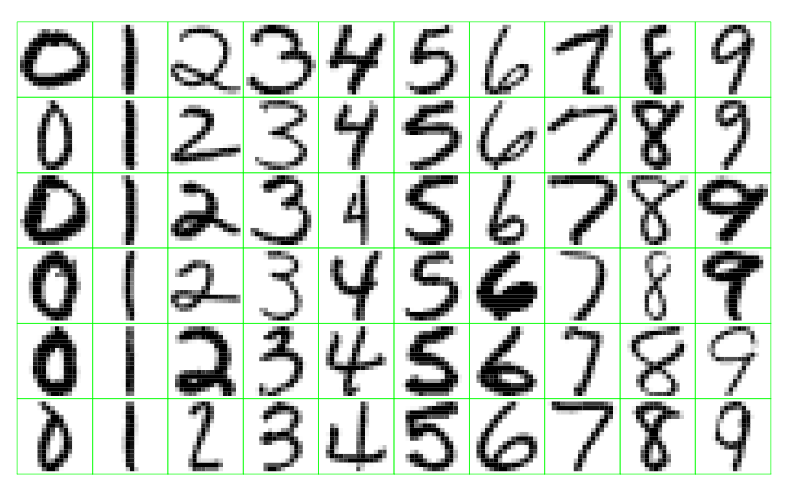
\includegraphics{digits.png}

\end{block}

\end{frame}

\begin{frame}

\begin{block}{Email classification (spam detection):}

The goal is to build a spam filter. This filter can based on the
frequencies of words and characters in emails. The table below show the
average percentage of words or characters in an email message, based on
4601 emails of which 1813 were classified as a spam.

\begin{longtable}[]{@{}lrrrrrr@{}}
\toprule
& you & free & george & ! & \$ & edu\tabularnewline
\midrule
\endhead
not spam & 1.27 & 0.07 & 1.27 & 0.11 & 0.01 & 0.29\tabularnewline
spam & 2.26 & 0.52 & 0.00 & 0.51 & 0.17 & 0.01\tabularnewline
\bottomrule
\end{longtable}

\end{block}

\end{frame}

\begin{frame}

\begin{block}{What makes a Nobel Prize winner?}

Perseverance, luck, skilled mentors or simply chocolate consumption? An
article published in the New England Journal of Medicine have concluded
with the following:

\begin{quote}
Chocolate consumption enhances cognitive function, which is a sine qua
non for winning the Nobel Prize, and it closely correlates with the
number of Nobel laureates in each country. It remains to be determined
whether the consumption of chocolate is the underlying mechanism for the
observed association with improved cognitive function.
\end{quote}

The figure shows the number of Nobel Laureates per 10 million population
against countries' annual per capita chocolate consumption.

You can read the article
\href{http://www.nejm.org/doi/full/10.1056/NEJMon1211064}{here} and a
informal review of the article
\href{https://blogs.scientificamerican.com/the-curious-wavefunction/chocolate-consumption-and-nobel-prizes-a-bizarre-juxtaposition-if-there-ever-was-one/}{here}.

\end{block}

\end{frame}

\begin{frame}

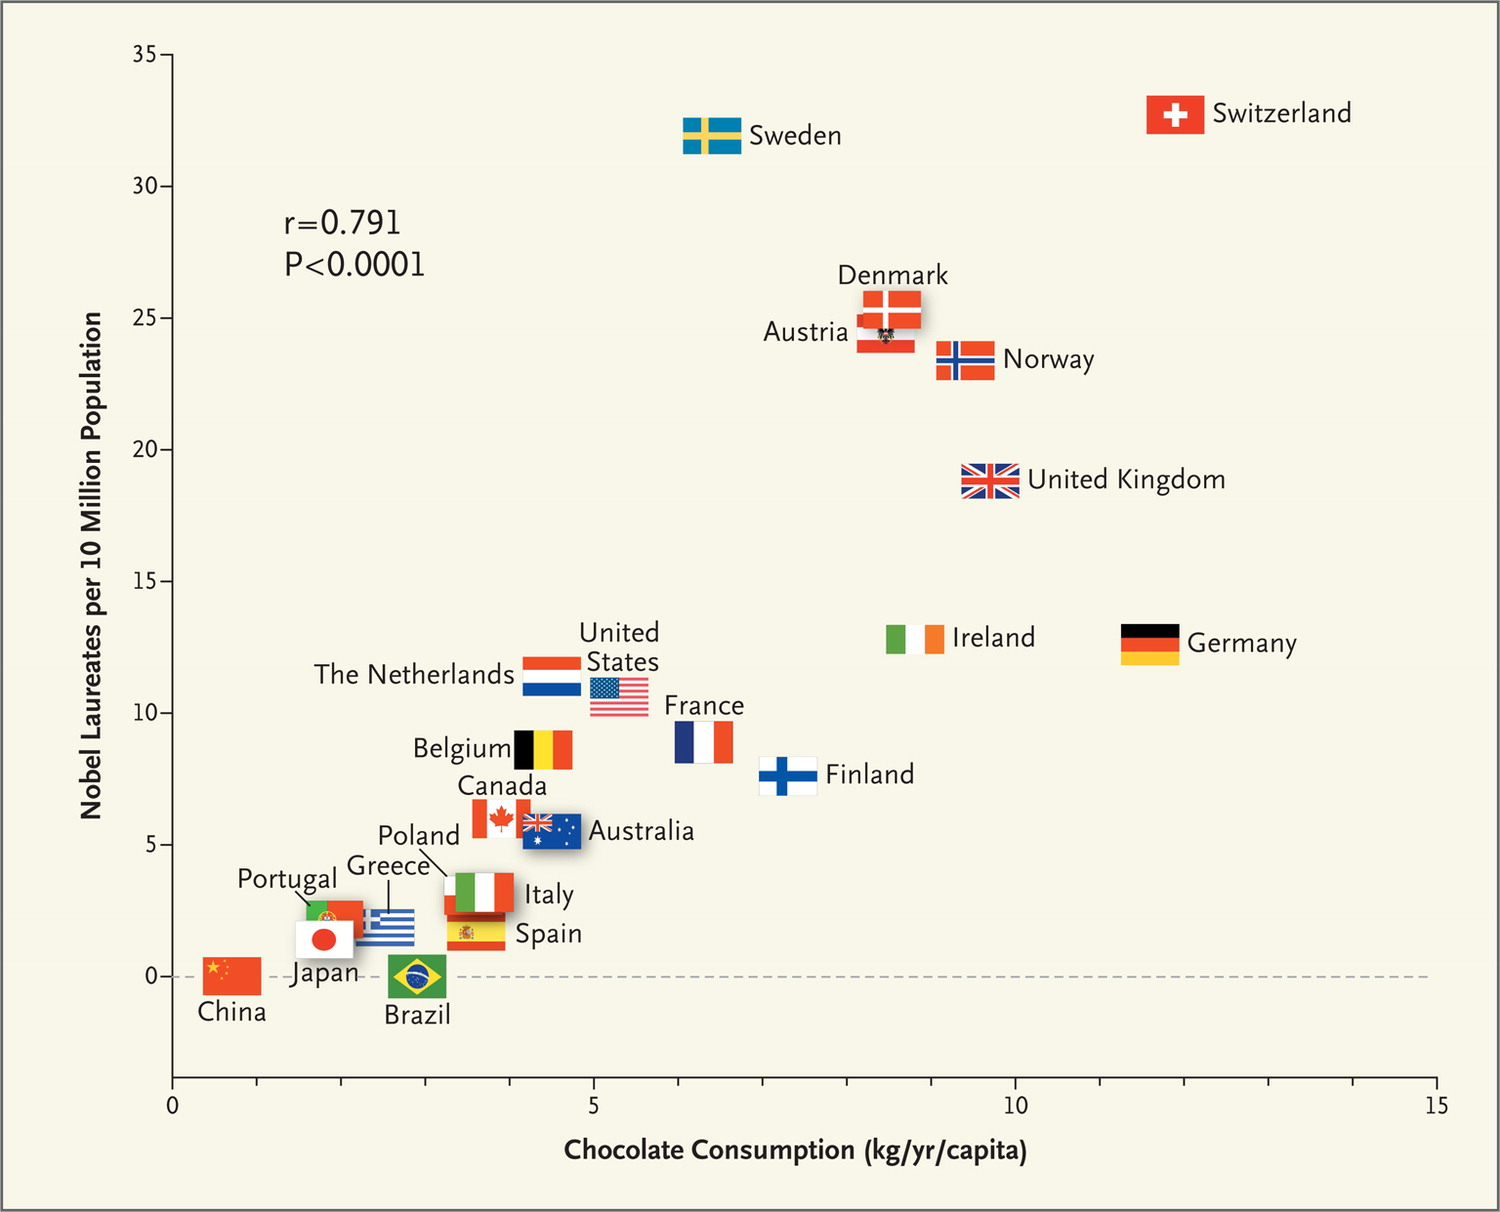
\includegraphics{chocolate.jpeg}

\end{frame}

\begin{frame}

\begin{block}{Were there common underlying aims and elements of these
examples of statistical learning?}

\begin{itemize}
\tightlist
\item
  To predict the price of a stock 3 months from now, based on company
  performance measures and economic data.
\item
  To identify the risk factors for developing diabetes based on diet,
  physical activity, family history and body measurements.
\item
  The goal is to build a spam filter.
\item
  To predict whether someone will suffer a heart attack on the basis of
  demographic, diet and clinical measurements.
\item
  To identify the numbers in a handwritten ZIP code, from a digitized
  image.
\item
  What makes a Nobel Prize winner? Perseverance, luck, skilled mentors
  or simply chocolate consumption?
\end{itemize}

\end{block}

\end{frame}

\begin{frame}{The Supervised Learning Problem}

\textcolor{blue}{\emph{Starting point}}:

\begin{itemize}
\item
  Outcome measurement \(Y\) (also called dependent variable, response,
  target).
\item
  Vector of \(p\) predictor measurements \emph{X} (also called inputs,
  regressors, covariates, features, independent variables).
\item
  In the \textbf{regression problem}, \(Y\) is quantitative (e.g price,
  blood pressure).
\item
  In the \textbf{classification problem}, \(Y\) takes values in a
  finite, unordered set (survived/died, digit 0-9, cancer class of
  tissue sample).
\item
  We have training data \((x_1, y_1), \ldots , (x_N , y_N )\). These are
  observations (examples, instances) of these measurements.
\end{itemize}

\end{frame}

\begin{frame}

\begin{block}{Supervised learning and its objectives}

Our data set (training set) consists of \(n\) measurement of the
response variable \(Y\) and of \(p\) covariates \(x\):
\[(y_1, x_{11}, x_{12},\ldots, x_{1p}), (y_2, x_{21},\ldots, x_{2p}), \ldots, (y_n, x_{n1}, x_{n2},\ldots, x_{np}).\]
\(~\)

On the basis of the \emph{training data} we would like to:

\begin{itemize}
\item
  \textbf{Accurately predict} unseen test cases.
\item
  \textbf{Understand} which input affects the outcomes, and how.
\item
  \textbf{Assess the quality} of your predictions and inference.
\end{itemize}

\end{block}

\end{frame}

\begin{frame}

Supervised learning examples (we will study):

\begin{itemize}
\tightlist
\item
  Linear regression (M3), Logistic regression (M4), Generalized additive
  models (M7)
\item
  Classification trees, bagging, boosting (M8), K-nearest neighbor
  classifier (M2, M4)
\item
  Support vector machines (M9)
\end{itemize}

\end{frame}

\begin{frame}{The Unsupervised Learning Problem}

\begin{itemize}
\item
  There is \textbf{no outcome variable} \(y\), just a set of predictors
  (features) \(x_i\) measured on a set of samples.
\item
  Objective is more fuzzy -- find (hidden) patterns or groupings in the
  data - in order to \emph{gain insight and understanding}. There is no
  \emph{correct} answer.
\item
  Difficult to know how well your are doing.
\item
  Different from supervised learning, but can be useful as a
  pre-processing step for supervised learning.
\end{itemize}

Examples in the course:

\begin{itemize}
\tightlist
\item
  Clustering (M10)
\item
  Principal component analysis (M10)
\end{itemize}

\end{frame}

\begin{frame}{Semi-supervised learning}

(Not considered in this course)

\begin{itemize}
\item
  Our data set consists of a input data, and some of the data has
  labelled responses.
\item
  This situation can for example occur if the measurement of input data
  is cheap, while the output data is expensive to collect.
\item
  Classical solutions (likelihood-based) to this problem exists in
  statistics (missing at random observations).
\end{itemize}

\end{frame}

\begin{frame}{Task}

Find examples to explain the difference between supervised and
unsupervised learning.

\begin{itemize}
\item
\item
\item
\end{itemize}

\end{frame}

\begin{frame}{Overall philosophy}

It is important to understand the ideas behind the various techniques,
in order to know how and when to use them.

\begin{itemize}
\item
  One has to understand the simpler methods first, in order to grasp the
  more sophisticated ones.
\item
  It is important to accurately assess the performance of a method, to
  know how well or how badly it is working
\end{itemize}

\(\rightarrow\) \textbf{Simpler methods often perform as well as fancier
ones!}

\begin{itemize}
\item
  This is an exciting research area, having important applications in
  science, industry and finance.
\item
  Statistical learning is a fundamental ingredient in the training of a
  modern data scientist.
\end{itemize}

\end{frame}

\begin{frame}{Statistical Learning vs.~Machine Learning}

\begin{itemize}
\item
  Machine learning arose as a subfield of Artificial Intelligence.
\item
  Statistical learning arose as a subfield of Statistics.
\item
  There is much overlap --- both fields focus on supervised and
  unsupervised problems:

  \begin{itemize}
  \tightlist
  \item
    Machine learning has a greater emphasis on large scale applications
    and prediction accuracy.
  \item
    Statistical learning emphasizes models and their interpretability,
    and precision and uncertainty.
  \end{itemize}
\item
  The distinction has become more and more blurred, and there is a great
  deal of ``cross-fertilization''.
\item
  Machine learning has the upper hand in Marketing!
\end{itemize}

\end{frame}

\begin{frame}

\begin{block}{Naming convention}

\begin{longtable}[]{@{}ll@{}}
\toprule
\begin{minipage}[b]{0.47\columnwidth}\raggedright\strut
Statistical learning\strut
\end{minipage} & \begin{minipage}[b]{0.47\columnwidth}\raggedright\strut
Machine learning\strut
\end{minipage}\tabularnewline
\midrule
\endhead
\begin{minipage}[t]{0.47\columnwidth}\raggedright\strut
model\strut
\end{minipage} & \begin{minipage}[t]{0.47\columnwidth}\raggedright\strut
network, graph, mapping\strut
\end{minipage}\tabularnewline
\begin{minipage}[t]{0.47\columnwidth}\raggedright\strut
fit, estimate\strut
\end{minipage} & \begin{minipage}[t]{0.47\columnwidth}\raggedright\strut
learn\strut
\end{minipage}\tabularnewline
\begin{minipage}[t]{0.47\columnwidth}\raggedright\strut
covariates, inputs, independent variables, predictors\strut
\end{minipage} & \begin{minipage}[t]{0.47\columnwidth}\raggedright\strut
features, predictors\strut
\end{minipage}\tabularnewline
\begin{minipage}[t]{0.47\columnwidth}\raggedright\strut
response, output, dependent variable\strut
\end{minipage} & \begin{minipage}[t]{0.47\columnwidth}\raggedright\strut
output, target\strut
\end{minipage}\tabularnewline
\begin{minipage}[t]{0.47\columnwidth}\raggedright\strut
data set\strut
\end{minipage} & \begin{minipage}[t]{0.47\columnwidth}\raggedright\strut
training data\strut
\end{minipage}\tabularnewline
\bottomrule
\end{longtable}

Remark: not an exhaustive list, and many terms are used in the same way
on both fields.

\end{block}

\end{frame}

\begin{frame}

\begin{itemize}
\item
  There is a controversy and some scepticism against ``too fancy'' ML
  methods.
\item
  Criticism: ML often re-invents existing methods and names them
  differently, but often without awareness of existing methods in
  statistics.
\item
  Almost weekly new literature that delivers comparison. Often, the
  ``simple'' statistcal methods ``win''.
\end{itemize}


\includegraphics{ML_vs_stat.png}

\end{frame}

\begin{frame}

\begin{block}{What is the aim in statistical learning?}

Assume:

\begin{itemize}
\tightlist
\item
  we observe one \emph{quantitative} response \(Y\) and
\item
  \(p\) different predictors \(x_1, x_2,... , x_p\).
\end{itemize}

We assume that there is a function \(f\) that relates the response and
the predictor variables: \[ Y = f(x) + \varepsilon,\] where
\(\varepsilon\) is a random error term with mean 0 and independent of
\(x\).

\end{block}

\end{frame}

\begin{frame}{Example 1}

\includegraphics{../../ISLR/Figures/Chapter2/2.1.png}

\end{frame}

\begin{frame}{Example 2}

\includegraphics{../../ISLR/Figures/Chapter2/2.2.png}

\end{frame}

\begin{frame}

There are two main reasons for estimating \(f\): \textbf{Prediction} and
\textbf{Inference}.

\end{frame}

\begin{frame}

\begin{block}{Prediction}

Based on observed data the aim is to build a model that as accurately as
possible can predict a response given new observations of the
covariates: \[\hat{Y} = \hat{f}(x).\] Here \(\hat{f}\) represents the
estimated \(f\) and \(\hat{Y}\) represents the prediction for \(Y\). In
this setting our estimate of the function \(f\) is treated as a
\textbf{black box and is not of interest}. Our focus is on the
prediction for \(Y\), hence prediction accuracy is important.

\end{block}

\end{frame}

\begin{frame}

There are two quantities which influence the accuracy of \(\hat{Y}\) as
a prediction of \(Y\): the reducible and the irreducible error.

\begin{itemize}
\tightlist
\item
  The \emph{reducible error} has to do with our estimate \(\hat{f}\) of
  \(f\). This error can be reduced by using the most \emph{appropriate}
  statistical learning technique.
\item
  The \emph{irreducible error} comes from the error term \(\varepsilon\)
  and cannot be reduced by improving \(f\). This is related to the
  unobserved quantities influencing the response and possibly the
  randomness of the situation.
\end{itemize}

\begin{block}{Q: If there were a \emph{deterministic} relationship
between the response and a set of predictors, would there then be both
reducible and irreducible error?}

\end{block}

\end{frame}

\begin{frame}

\begin{block}{A:}

If we know all predictors and the (deterministic) connection to the
reponse, and there is no random error added, then we will have no
irreducible error. If there is a deterministic relationship, but we
don't know all predictor values, then the non-observed predictors will
give us irreducible error.

So, very seldom (maybe only in synthetic examples?) that there is only
reducible error present.

\end{block}

\end{frame}

\begin{frame}

\begin{block}{Inference}

Based on observed data the aim is to \emph{understand} how the response
variable is affected by the various predictors (covariates).

In this setting we will not use our estimated function \(\hat{f}\) to
make predictions but to \emph{understand} how \(Y\) changes as a
function of \(x_1, x_2, ..., x_p\).

The \emph{exact form} of \(\hat{f}\) is of \emph{main interest}.

\begin{itemize}
\tightlist
\item
  Which predictors are associated with the response?
\item
  What is the relationship between the response and each predictor?
\item
  Can the relationship be linear, or is a more complex model needed?
\end{itemize}

\end{block}

\end{frame}

\begin{frame}

\begin{block}{Regression and classification}

\textbf{Regression} predicts a value from a continuous set.

Example: Predict the profit given the amount of money spend on
advertising.

\textbf{Classification} predicts the class membership.

Example: Given blood pressure, weight and hip ratio predict if a patient
suffers from diabetes (yes/no).

\begin{block}{Q:}

Give an example of one regression and one classification problem
(practical problem with data set available) that you would like to study
in this course.

\end{block}

\begin{block}{A:}

See examples in M1 and M2.

\end{block}

\end{block}

\end{frame}

\begin{frame}{Models and methods}

\begin{block}{Parametric Methods}

Parametric methods build on an assumption about the form or shape of the
function \(f\).

The multiple linear model (M3) is an example of a parametric method. We
here assume that the response variable is a linear combination of the
covariates with some added noise
\[f(x) = \beta_0 + \beta_1 x_1 + ... + \beta_p x_p+\varepsilon.\] By
making this assumption, the task simplifies to finding estimates of the
\(p+1\) coefficients \(\beta_0, \beta_1, .. ,\beta_p\). To do this we
use the training data to fit the model, such that
\[Y \approx \hat{\beta_0} + \hat{\beta_1} x_1 + ... + \hat{\beta_p} x_p.\]

\end{block}

\end{frame}

\begin{frame}

Fitting a parametric models is thus done in two steps:

\begin{enumerate}
\def\labelenumi{\arabic{enumi}.}
\tightlist
\item
  Select a form for the function \(f\).\\
\item
  Estimate the unknown parameters in \(f\) using the training set.
\end{enumerate}

\end{frame}

\begin{frame}

\begin{block}{Non-parametric methods}

Non-parametric methods seek an estimate of \(f\) that gets close to the
data points, but without making explicit assumptions about the form of
the function \(f\).

The \(K\)-nearest neighbour algorithm is an example of a non-parametric
model. Used in classification, this algorithm predicts a class
membership for a new observation by making a majority vote based on its
\(K\) nearest neighbours. We will discuss the \(K\)-nearest neighbour
algorithm later in this module.

\end{block}

\end{frame}

\begin{frame}

\begin{block}{Q: What are advantages and disadvantages of parametric and
non-parametric methods?}

Hints: interpretability, amount of data needed, complexity, assumptions
made, prediction accuracy, computational complexity, over/under-fit.

\end{block}

\end{frame}

\begin{frame}

\begin{block}{A: Parametric methods}

\begin{longtable}[]{@{}ll@{}}
\toprule
\begin{minipage}[b]{0.47\columnwidth}\raggedright\strut
Advantages\strut
\end{minipage} & \begin{minipage}[b]{0.47\columnwidth}\raggedright\strut
Disadvantages\strut
\end{minipage}\tabularnewline
\midrule
\endhead
\begin{minipage}[t]{0.47\columnwidth}\raggedright\strut
Simple to use and easy to understand\strut
\end{minipage} & \begin{minipage}[t]{0.47\columnwidth}\raggedright\strut
The function \(f\) is constrained to the specified form.\strut
\end{minipage}\tabularnewline
\begin{minipage}[t]{0.47\columnwidth}\raggedright\strut
Requires little training data\strut
\end{minipage} & \begin{minipage}[t]{0.47\columnwidth}\raggedright\strut
The assumed function form of \(f\) will in general not match the true
function, potentially giving a poor estimate.\strut
\end{minipage}\tabularnewline
\begin{minipage}[t]{0.47\columnwidth}\raggedright\strut
Computationally cheap\strut
\end{minipage} & \begin{minipage}[t]{0.47\columnwidth}\raggedright\strut
Limited complexity\strut
\end{minipage}\tabularnewline
\bottomrule
\end{longtable}

\end{block}

\end{frame}

\begin{frame}

\begin{block}{A: Non-parametric methods}

\begin{longtable}[]{@{}ll@{}}
\toprule
\begin{minipage}[b]{0.47\columnwidth}\raggedright\strut
Advantages\strut
\end{minipage} & \begin{minipage}[b]{0.47\columnwidth}\raggedright\strut
Disadvantages\strut
\end{minipage}\tabularnewline
\midrule
\endhead
\begin{minipage}[t]{0.47\columnwidth}\raggedright\strut
Flexible: a large number of functional forms can be fitted\strut
\end{minipage} & \begin{minipage}[t]{0.47\columnwidth}\raggedright\strut
Can overfit the data\strut
\end{minipage}\tabularnewline
\begin{minipage}[t]{0.47\columnwidth}\raggedright\strut
No strong assumptions about the underlying function are made\strut
\end{minipage} & \begin{minipage}[t]{0.47\columnwidth}\raggedright\strut
Computationally more expensive as more parameters need to be
estimated\strut
\end{minipage}\tabularnewline
\begin{minipage}[t]{0.47\columnwidth}\raggedright\strut
Can often give good predictions\strut
\end{minipage} & \begin{minipage}[t]{0.47\columnwidth}\raggedright\strut
Much data is required to estimate (the complex) \(f\).\strut
\end{minipage}\tabularnewline
\bottomrule
\end{longtable}

\end{block}

\end{frame}

\begin{frame}{Prediction accuracy vs.~interpretability}

(we are warming up to the bias--variance trade--off)

\textbf{Inflexible}, or rigid, methods are methods which have strong
restrictions on the shape of \(f\).

Examples:

\begin{itemize}
\tightlist
\item
  Linear regression (M3)
\item
  Linear discriminant analysis (M4)
\item
  Subset selection and lasso (M6)
\end{itemize}

\textbf{Flexible} methods have less restriction on the shape of \(f\).

Examples:

\begin{itemize}
\tightlist
\item
  KNN classification (M2, M4), KNN regression, Smoothing splines (M7)
\item
  Bagging and boosting (M8), support vector machines (M9)
\item
  Neural networks (M11)
\end{itemize}

\end{frame}

\begin{frame}

The choice of a flexible or inflexible method depends on the goal in
mind.

If the aim is inference an inflexible model, which is easy to
understand, will be preferred. On the other side, if we want to make as
accurate predictions as possible, we are not concerned about the shape
of \(f\). A flexible method can be chosen, at the cost of model
interpretability, and we treat \(f\) like a black box.

\textbf{Overfitting} occurs when the estimated function \(f\) is too
closely fit to the observed data points.

\textbf{Underfitting} occurs when the estimated function \(f\) is too
rigid to capture the underlying structure of the data.

We illustrate this by a toy example using polynomial regression.

\end{frame}

\begin{frame}

\begin{block}{Polynomial regression example}

Consider a covariate \(x\) observed on a grid on the real line from -2
to 4, equally spaced at 0.1, giving \(n=61\) observations.

\includegraphics{2StatLearn_files/figure-beamer/data-1.pdf}

\end{block}

\end{frame}

\begin{frame}

Assume a theoretical relationship between reponse \(Y\) and covariate
\(x\):

\[ Y=x^2 + \varepsilon\] Where \(\varepsilon\) is called an error (or
noise) term, and is simulated to from a normal distribution with mean 0
and standard deviation 2.

We call \(Y=x^2\) the \emph{truth}.

The added error is used as a substitue for all the unobserved variables
that are not in our equation, but that might influence \(Y\). This means
that we are not looking at a purely \emph{deterministic} relationship
between \(x\) and \(Y\), but allow for randomness.

\end{frame}

\begin{frame}

\includegraphics{2StatLearn_files/figure-beamer/truth-1.pdf}

\end{frame}

\begin{frame}

Next, we want to fit a function to the observations \emph{without}
knowing the true relationship, and we have tried different parametric
polynomial functions.

\begin{itemize}
\tightlist
\item
  {{[}poly1: upper left{]}}: The {red} line shows a simple linear model
  of the form \(\beta_0+\beta_1 x\) fitted to the observations. This
  line clearly \emph{underfits} the data. We see that this function is
  unable to capture that quadratic nature of the data.
\item
  {{[}poly2: upper right{]}}: The {orange} line shows a quadratic
  polynomial fit to the data, of the form
  \(\beta_0+\beta_1 x +\beta_2 x^2\). We see that this function fits
  well and looks almost identically as the true function.
\item
  {{[}poly10: lower left{]}}: The {pink} line shows a polynomial of
  degree 10 fit to the data, of the form
  \(\beta_0+\beta_1 x +\beta_2 x^2+\cdots +\beta_{10}x^{10}\). The
  function captures the noise instead of the underlying structure of the
  data. The function \emph{overfits} the data.
\item
  {{[}poly20: lower right{]}}: The {purple} line shows a polynomial of
  degree 20 fit to the data, of the form
  \(\beta_0+\beta_1 x +\beta_2 x^2+\cdots +\beta_{20}x^{20}\). The
  function captures the noise instead of the underlying structure of the
  data. The function \emph{overfits} the data.
\end{itemize}

We will discuss polynomial regression in M7.

\end{frame}

\begin{frame}

\includegraphics{2StatLearn_files/figure-beamer/overunderfit-1.pdf}

\end{frame}

\begin{frame}

\textbf{Why comparing regressions with different degrees of
polynomials?} We will study several methods that includes a parameter
controlling the flexibility of the model fit - so generalizations of our
example with degrees for the polynomials. The \(K\) in K-nearest
neighour is such a parameter. We need to know how to choose this
flexibility parameter.

\end{frame}

\begin{frame}

\textbf{Q}: The coloured curves are our estimates for the functional
relationship between \(x\) and \(Y\). We will next work with the
following questions.

\begin{itemize}
\tightlist
\item
  Which of the coloured curves does the best job? Rank the curves.
\end{itemize}

Now, disregard the poly2 orange curve, and only consider the red, pink
and puple curves.

\begin{itemize}
\tightlist
\item
  Assume that we collect new data of \(Y\) (but with new normally
  distributed errors added) - and estimate new curves. Which of the
  coloured curves would \emph{on average} give the best performance?
\item
  What did you here choose to define as ``best performance''?
\end{itemize}

\end{frame}

\begin{frame}

\includegraphics{2StatLearn_files/figure-beamer/plottingM-1.pdf}

Kept x fixed and drew new errors 100 times. The 100 fitted curves shown.
The black line is the true \(y=x^2\) curve

\end{frame}

\begin{frame}

\begin{block}{Loss function}

We now focus on prediction.

\textbf{Q:} How can we measure the \emph{loss} between a predicted
response \(\hat{y}_i\) and the observed response \(y_i\)?

\textbf{A:} Possible loss functions are:

\begin{itemize}
\tightlist
\item
  absolute loss (L1 norm): \(\mid y_i-\hat{y}_i\mid\)
\item
  quadratic loss (L2 norm): \((y_i-\hat{y}_i)^2\)
\item
  0/1 loss (categorical \(y\)): loss=0 if \(\hat{y_i}=y_i\) and 1 else
\end{itemize}

Issues: robustness, stability, mathematical aspect.

We will use quadratic loss now.

\end{block}

\end{frame}

\begin{frame}

\begin{block}{Assessing model accuracy - and quality of fit}

\textbf{Q:} For regression (and classification) in general: will there
be \emph{one} method that dominates all others?

\textbf{A:} No method dominates all others over all possible data sets.

\begin{itemize}
\tightlist
\item
  That is why we need to learn about many different methods.
\item
  For a given data set we need to know how to decide which method
  produces the \emph{best} results.
\item
  How close is the predicted response to the true response value?
\end{itemize}

\end{block}

\end{frame}

\begin{frame}

\begin{block}{Training MSE}

In regression, where we assume \(Y = f(x) + \varepsilon\), and
\(\hat{f}(x_i)\) gives the predicted response at \(x_i\), a popular
measure is the \emph{training MSE} (mean squared error): mean of squared
differences between prediction and truth for the training data (the same
values that were used to estimate \(f\)):
\[ \text{MSE}_{\text{train}}=\frac{1}{n}\sum_{i=1}^n (y_i-\hat{f}(x_i))^2\]

But, really - we are \emph{not} interested in how the method works on
the training data (and often we have designed the method to work good on
the training data already), we want to know how good the method is when
we use it on \emph{previously unseen test data}, that is, data that we
may observe in the future.

\end{block}

\end{frame}

\begin{frame}

Example:

\begin{itemize}
\tightlist
\item
  we don't want to predict last weeks stock price, we want to predict
  the stock price next week.
\item
  we don't want to predict if a patient in the training data has
  diabetes, we want to predict if a new patient has diabetes.
\end{itemize}

\end{frame}

\begin{frame}

\includegraphics{2StatLearn_files/figure-beamer/trainMSE-1.pdf}

\textbf{Q}: Based on the training MSE - which model fits the data the
best?

Polynomial example: fitted order 1-20 polynomial when the truth is order
2. Left: one repetition, right: 100 repetitions of the training set.

(But, how was these graphs made? Want to see the R code? You can see the
code by looking at the 2StatLearn.Rmd file located at the same place as
you found this file.)

\end{frame}

\begin{frame}

\begin{block}{Test MSE}

Simple solution: we fit (estimate \(\hat(f)\)) from different models
using the training data (maybe my minimizing the training MSE), but we
choose the \emph{best} model using a separate \emph{test set} - by
calculating the \emph{test MSE} for a set of \(n_0\) test observations
\((x_{0j},y_{0j})\):

\[ \text{MSE}_{\text{test}}=\frac{1}{n_0}\sum_{j=1}^{n_0} (y_{0j}-\hat{f}(x_{0j}))^2\]

Alternative notation: \[\text{Ave}(y_0-\hat{f}(x_0))^2\] (taking the
average over all available test observations).

\end{block}

\end{frame}

\begin{frame}

\textbf{Q:} What if we do not have access to test data?

\textbf{A:} In Module 5 we will look into using \emph{cross validation}
to mimic the use of a test set.

\textbf{Q:} But, can we instead just use the training data MSE to choose
a model? A low training error should also give a low test error?

\textbf{A:} Sadly no, if we use a flexible model we will look at several
cases where a low training error is a sign of overfitting, and will give
a high test error. So, the training error is not a good estimator for
the test error because it does not properly account for model
complexity.

\end{frame}

\begin{frame}

\includegraphics{2StatLearn_files/figure-beamer/traintestMSE-1.pdf}

Polynomial example: fitted order 1-20 when the truth is order 2. Left:
one repetition, right: 100 repetitions for the testMSE.

\textbf{Q}: Based on the test MSE - which model fits the data the best?

\end{frame}

\begin{frame}

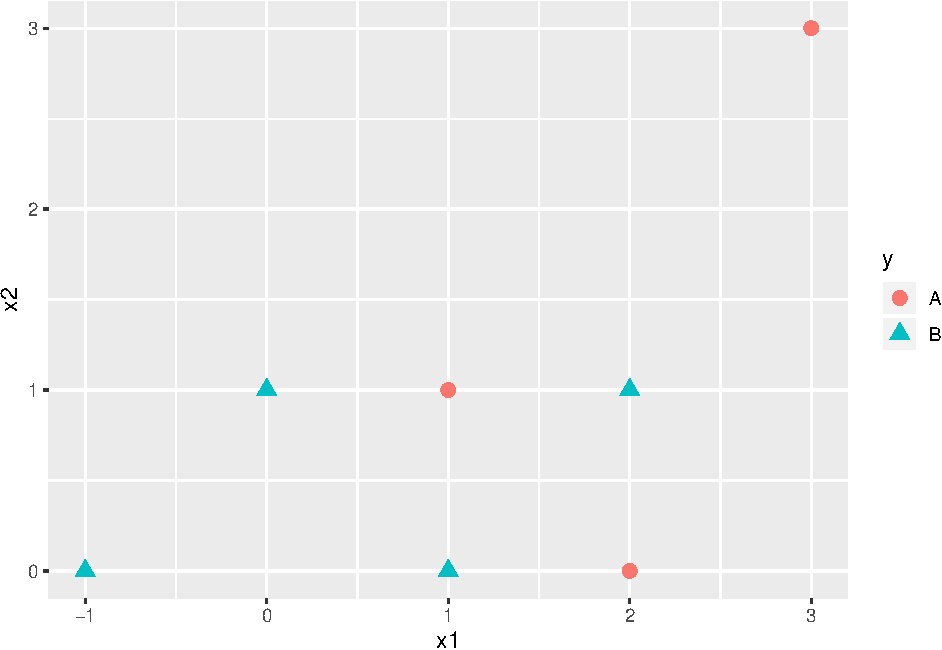
\includegraphics{2StatLearn_files/figure-beamer/unnamed-chunk-1-1.pdf}

\textbf{A}: If choosing flexibility based on training MSE=poly20 wins,
if choose flexibility based on test MSE=poly 2 wins.

Polynomial example: fitted order 1-20 when the truth is order 2. Upper:
trainMSE, lower: testMSE. Left: one repetition, right: 100 repetitions.

\end{frame}

\begin{frame}

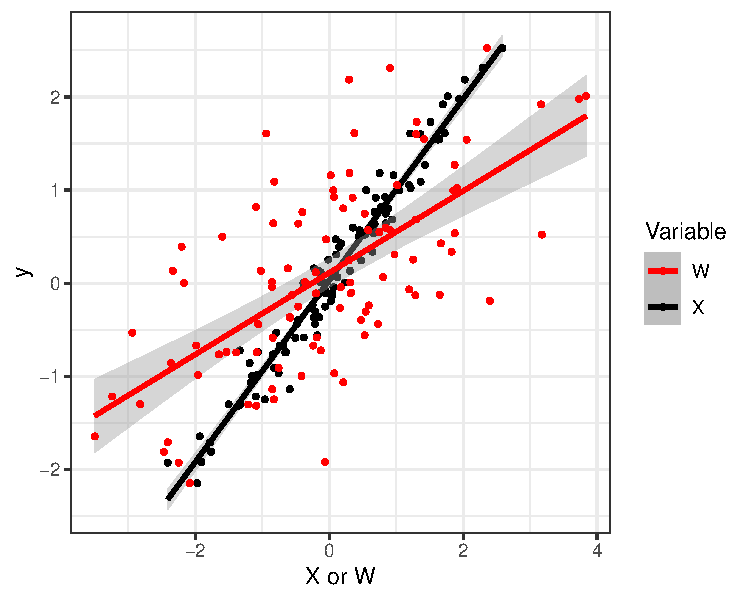
\includegraphics{2StatLearn_files/figure-beamer/unnamed-chunk-2-1.pdf}

Boxplot of the 100 repetitions (polynomial experiment). Observe the
U-shaped for the test error.

\textbf{Q}: What can you read of the boxplot? Anything new compared to
the previous plots?

\end{frame}

\begin{frame}

\textbf{A}:

Same data as above, but now presented jointly for training and test MSE,
to focus on location and variability:

Boxplot:

\begin{itemize}
\tightlist
\item
  black line=median,
\item
  box from 1 to 3rd quantile,
\item
  IQR=inter quartile range= width of box
\item
  whiskers to min and max, except when more than 1.5 times IQR from box,
  then marked as outlier with points.
\end{itemize}

\end{frame}

\begin{frame}

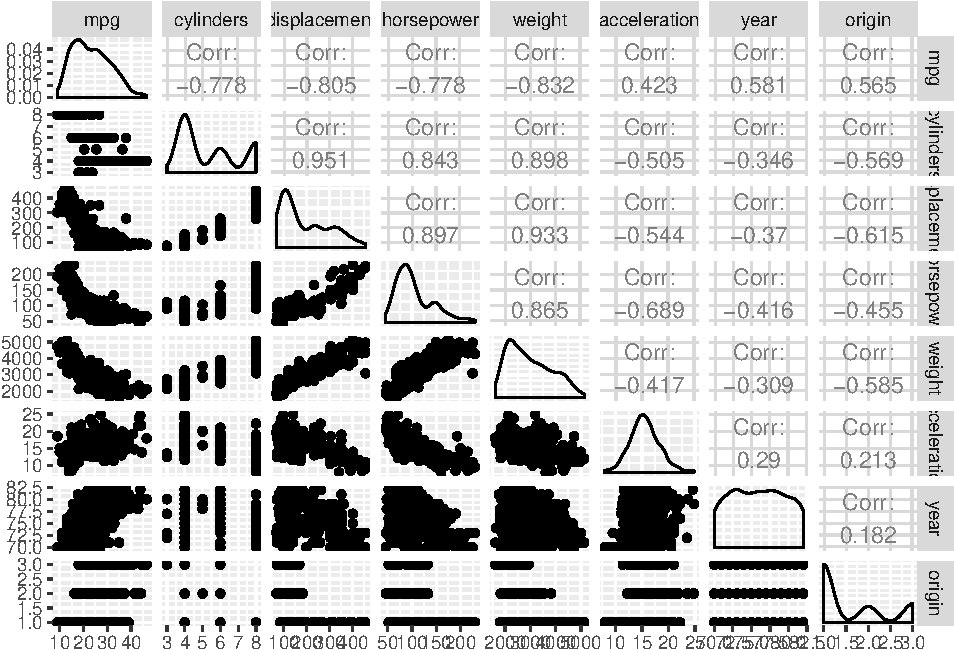
\includegraphics{2StatLearn_files/figure-beamer/unnamed-chunk-3-1.pdf}

Mean of 100 repetitions (polynomial example). Observe U-shape.

\textbf{Next: We leave the trainMSE and try to understand what makes up
the testMSE curve - two competing properties!}

\end{frame}

\begin{frame}{The Bias-Variance trade-off}

Assume that we have fitted a \emph{regression} curve
\(Y = f(x) + \varepsilon\) to our training data, which consist of
independent observation pairs \(\{x_i, y_i\}\) for \(i=1,..,n\). (Yes,
only one covariate \(x\).)

We assume that \(\varepsilon\) is an unobserved random variable that
adds noise to the relationship between the response variable and the
covariates and is called the random error, and that the random errors
have mean zero and constant variance \(\sigma^2\) for all values of
\(x\).

This noise is used as a substitute for all the unobserved variables that
is not in our equation, but that influences \(Y\).

Assume that we have used our training data to produce a fitted curve,
denoted by \(\hat{f}\).

\end{frame}

\begin{frame}

We want to use \(\hat{f}\) to make a prediction for a new observation at
\(x_0\), and are interested in the error associated with this
prediction. The predicted response value is then \(\hat{f}(x_0)\).

The \emph{expected test mean squared error (MSE) at \(x_0\)} is defined
as: \[\text{E}[Y - \hat{f}(x_0)]^2\]

Remark 1: yes, we could have called the new response \(Y_0\) instead of
\(Y\).\\
Remark 2: compare this to the test MSE for the polynomical example -
observe that here we have the \emph{theoretical version} where we have
replaced the average with the mathematical mean.

\end{frame}

\begin{frame}

This expected test MSE can be decomposed into three terms
\[\text{E}[Y - \hat{f}(x_0)]^2 = \text{E}[Y^2 + \hat{f}(x_0)^2 - 2 Y \hat{f}(x_0)] \]
\[= \text{E}[Y^2] + \text{E}[\hat{f}(x_0)^2] - \text{E}[2Y \hat{f}(x_0)]\]
\[= \text{Var}[Y] + \text{E}[Y]^2 + \text{Var}[\hat{f}(x_0)] + \text{E}[\hat{f}(x_0)]^2 - 2 \text{E}[Y]\text{E}[\hat{f}(x_0)] \]
\[= \text{Var}[Y]+f(x_0)^2+\text{Var}[\hat{f}(x_0)]+\text{E}[\hat{f}(x_0)]^2-2f(x_0)\text{E}[\hat{f}(x_0)]\]
\[= \text{Var}[Y]+\text{Var}[\hat{f}(x_0)]+(f(x_0)-\text{E}[\hat{f}(x_0)])^2\]
\[= \text{Var}(\varepsilon) +  \text{Var}[\hat{f}(x_0)]+[\text{Bias}(\hat{f}(x_0))]^2.\]

\textbf{Q}: what assumptions have we made in the derivation above?

\textbf{A}: classnotes.

\end{frame}

\begin{frame}

\[\text{E}[(Y - \hat{f}(x_0))^2]=\cdots=\text{Var}(\varepsilon) +  \text{Var}[\hat{f}(x_0)]+[\text{Bias}(\hat{f}(x_0))]^2\]

\begin{itemize}
\tightlist
\item
  First term: irreducible error, \(\text{Var}(\varepsilon)=\sigma^2\)
  and is always present unless we have measurements without error. This
  term cannot be reduced regardless how well our statistical model fits
  the data.
\item
  Second term: variance of the prediction at \(x_0\) or the expected
  deviation around the mean at \(x_0\). If the variance is high, there
  is large uncertainty associated with the prediction.
\item
  Third term: squared bias. The bias gives an estimate of how much the
  prediction differs from the true mean. If the bias is low the model
  gives a prediction which is close to the true value.
\end{itemize}

\end{frame}

\begin{frame}

\[\text{E}[(Y - \hat{f}(x_0))^2]=\cdots=\text{Var}(\varepsilon) +  \text{Var}[\hat{f}(x_0)]+[\text{Bias}(\hat{f}(x_0))]^2\]

This is the \textbf{expected test MSE}. We can think of this as the
average test MSE we would obtain if we repeatedly estimated \(f\) using
many training sets (as we did in our example), and then tested this
estimate at \(x_0\).

So, this is really \(\text{E}[(Y - \hat{f}(x_0))^2 \mid X=x_0]\) if we
also assume that \(X\) is a random variable.

The \textbf{overall expected test MSE} can we then compute by averaging
the expected test MSE at \(x_0\) over all possible values of \(x_0\)
(averaging with respect to frequency in test set), or mathematically by
the law of total expectation
\(\text{E} \{ \text{E}[(Y - \hat{f}(X))^2 \mid X]\}\) (also sometimes
referred to as the law of double expectations).

\end{frame}

\begin{frame}

\begin{block}{Polynomial example (cont.)}

\includegraphics{2StatLearn_files/figure-beamer/biasvarianceforx-1.pdf}

\textbf{Q:} Summarize the most important features of these plots.

For 4 different polynomial models (poly1,2,10 and 20), the squared bias,
variance, irreducible error and the total sum. Plots based on 100
simulations for the polynomial example.

\end{block}

\end{frame}

\begin{frame}

\includegraphics{2StatLearn_files/figure-beamer/biasvarianceforpoly-1.pdf}

\textbf{Q:} Summarize the most important features of these plots.

At 4 different values for \(x_0\), the squared bias, variance,
irreducible error and the total sum. Plots based on 100 simulations for
the polynomial example.

\end{frame}

\begin{frame}

\includegraphics{2StatLearn_files/figure-beamer/averageoverxs-1.pdf}

Overall version (averaging over 61 gridpoints of x).

\end{frame}

\begin{frame}

\begin{block}{Choosing the best model: observations}

When fitting a statistical model the aim is often to obtain the most
predictive model. There are often many candidate models, and the task is
to decide which model to choose.

\begin{itemize}
\tightlist
\item
  The observations used to fit the statistical model make up the
  training set. The training error is the average loss over the training
  sample.
\item
  As the complexity (and thus flexibility) of a model increases the
  model becomes more adaptive to underlying structures and the training
  error falls.
\item
  The test error is the prediction error over a test sample.
\item
  The test sample will have new observations which were not used when
  fitting the model. One wants the model to capture important
  relationships between the response variable and the covariates, else
  we will underfit. Recall the red line in the figure corresponding to
  the toy example above.
\end{itemize}

\end{block}

\end{frame}

\begin{frame}

This trade-off in selecting a model with the right amount of
complexity/flexibility is the \textbf{variance-bias trade-off}.

To summarize:

\begin{itemize}
\tightlist
\item
  inflexible models (with few parameters to fit) are easy to compute but
  may lead to a poor fit (high bias)
\item
  flexible (complex) models may provide more unbiased fits but may
  overfit the data (high variance)
\item
  there will be irreducible errors present
\end{itemize}

We will in Module 6 see that by choosing a biased estimator may be
better than an unbiased due to differences in variances, and in Module 8
see how methods as bagging, boosting and random forests can lower the
variance while prevailing a low bias.

\end{frame}

\begin{frame}

\includegraphics{../../ISLR/Figures/Chapter2/2.12.png}

\end{frame}

\begin{frame}{Classification}

(so far, regression setting - but how about model accuracy in
classification?)

\textbf{Set-up:} Training observations (independent pairs)
\(\{(x_1, y_1), ..., (x_n, y_n)\}\) where the response variable \(Y\) is
qualitative. E.g \(Y \in \mathcal{C} = \{0, 1, ..., 9\}\) or
\(Y \in \mathcal{C} = \{dog, cat,... ,horse\}\).

\textbf{Aim: } To \emph{build} a classifier \(f(x)\) that assigns a
class label from \(\mathcal{C}\) to a future unlabelled observation
\(x\) and to asses the \emph{uncertainty} in this classification.
Sometimes the role of the different predictors may be of main interest.

\textbf{Performance measure:} Most popular is the misclassification
error rate (training and test version).

\textbf{0/1-loss}: The misclassifications are given the loss 1 and the
correct classifications loss 0. (Quadratic loss is not used for
classification.)

\begin{block}{Q: Give an example of a classification problem.}

\end{block}

\end{frame}

\begin{frame}

\begin{block}{A: some examples earlier in this module, and new examples
will be added to the class notes.}

\end{block}

\end{frame}

\begin{frame}

\begin{block}{Synthetic example}

\begin{itemize}
\tightlist
\item
  The figure below shows a plot of 100 observations from two classes
  \(A\) (red dots) and \(B\) (turquoise dots),
\item
  simulated from a bivariate normal distribution with mean vectors
  \(\mu_A = (1, 1)^T\) and \(\mu_B = (3, 3)^T\) and a covariance matrix
  \(\Sigma_A = \Sigma_B = \begin{pmatrix} 2\hspace{2mm} 0 \\ 0 \hspace{2mm} 2 \end{pmatrix}\).
\item
  We want to find a rule to classify a new observation to class \(A\) or
  \(B\).
\end{itemize}

\end{block}

\end{frame}

\begin{frame}

\includegraphics{2StatLearn_files/figure-beamer/knn-1.pdf}

\end{frame}

\begin{frame}

\begin{block}{Training error rate}

the proportion of mistakes that are made if we apply our estimator
\(\hat{f}\) to the training observations, i.e.
\(\hat{y}_i=\hat{f}(x_i)\).
\[\frac{1}{n}\sum_{i=1}^n \text{I}(y_i \neq \hat{y}_i).\] Here I is the
indicator function (to give our 0/1 loss) which is defined as:
\[\text{I}(a\neq\hat{a}) = \begin{cases} 1 \text{ if } a \neq \hat{a} \\ 0 \text{ else } \end{cases}\]
The indicator function counts the number of times our model has made a
wrong classification. The training error rate is the fraction of
misclassifications made on our training set. A very low training error
rate may imply overfitting.

\end{block}

\end{frame}

\begin{frame}

\begin{block}{Test error rate}

Here the fraction of misclassifications is calculated when our model is
applied on a test set. From what we have learned about regression we can
deduce that this gives a better indication of the true performance of
the classifier (than the training error).
\[\text{Ave}(I(y_0\neq \hat{y}_0))\] where the average is over all the
test observations \((x_0,y_0)\).

We assume that a \emph{good} classifier is a classifier that has a
\emph{low} test error.

\end{block}

\end{frame}

\begin{frame}

\begin{block}{Bayes classifier}

Suppose we have a quantitative response value that can be a member in
one of \(K\) classes \(\mathcal{C} = \{c_1, c_2, ..., c_k, ..., c_K\}\).
Further, suppose these elements are numbered \(1, 2, ..., K\). The
probability of that a new observation \(x_0\) belongs to class \(k\) is
\[p_k(x_0) = \text{Pr}(Y=k | X=x_0), \quad k = 1, 2, ... K.\] This is
the conditional class probability: the probability that \(Y=k\) given
the observation \(x_0\). The \emph{Bayes classifier assigns an
observation to the most likely class}, given its predictor values.

This is best illustrated by a two-class example. Assume our response
value is to classified as belonging to one of the two groups
\(\{A, B\}\). A new observation \(x_0\) will be classified to \(A\) if
\(\text{Pr}(Y=A | X=x_0) > 0.5\) and to class \(B\) otherwise.

\end{block}

\end{frame}

\begin{frame}

\textbf{The Bayes classifier}

\begin{itemize}
\tightlist
\item
  has the \emph{smallest test error rate}.
\item
  However, we never (or very seldom) know the conditional distribution
  of \(Y\) given \(X\) for real data. Computing the Bayes classifier is
  thus impossible.
\item
  The class boundaries using the Bayes classifier is called the
  \emph{Bayes decision boundary}.
\item
  The overall Bayes error rate is given as
  \[1-\text{E}(\text{max} \text{Pr}(Y=j\mid X))\] where the expectation
  is over \(X\).
\item
  The Bayes error rate is comparable to the \emph{irreducible error} in
  the regression setting.
\end{itemize}

Next: \(K\)-nearest neighbor classifier estimates this conditional
distribution and then classifies a new observation based on this
estimated probability.

\end{frame}

\begin{frame}

\begin{block}{K-nearest neighbour classifier}

The \(K\)-nearest neighbour classifier (KNN) works in the following way:

\begin{itemize}
\tightlist
\item
  Given a new observation \(x_0\) it searches for the \(K\) points in
  our training data that are closest to it (Euclidean distance).
\item
  These points make up the neighborhood of \(x_0\), \(\mathcal{N}_0\).
\item
  The point \(x_0\) is classified by taking a majority vote of the
  neighbors.
\item
  That means that \(x_0\) is classified to the most occurring class
  among its neighbors
  \[\text{Pr}(Y=j | X = x_0) = \frac{1}{K} \sum_{i \in \mathcal{N}_0} I(y_i = j).\]
\end{itemize}

\end{block}

\end{frame}

\begin{frame}

We return to our synthetic data with \(X_1\) and \(X_2\) and two classes
\(A\) and \(B\):

\begin{itemize}
\tightlist
\item
  Assume we have a new observation \(X_0 = (x_{01}, x_{02})^T\) which we
  want to classify as belonging to the class \(A\) or \(B\).
\item
  To illustrate this problem we fit the \(K\)-nearest neighbor
  classifier to our simulated data set with \(K = 1, 3, 10\) and \(150\)
  and observe what happens.
\end{itemize}

In our plots, the small colored dots show the predicted classes for an
evenly-spaced grid. The lines show the decision boundaries. If our new
observation falls into the region within the red decision boundary, it
will be classified as \(A\). If it falls into the region within the
green decision boundary, it will be classified as \(B\).

\end{frame}

\begin{frame}

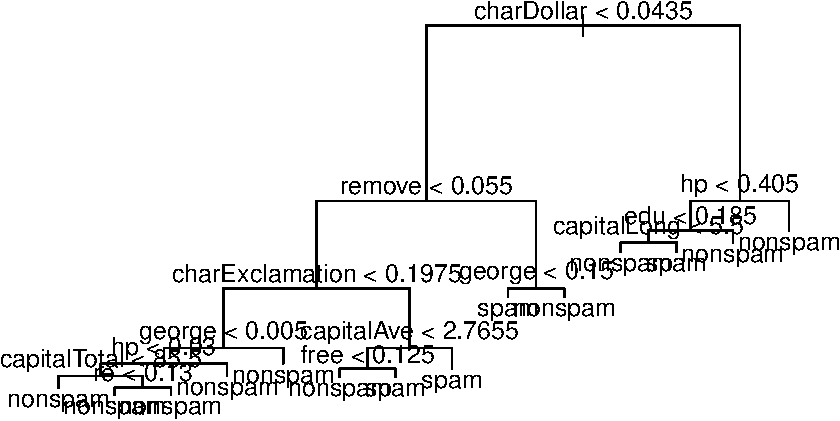
\includegraphics{2StatLearn_files/figure-beamer/unnamed-chunk-4-1.pdf}

\end{frame}

\begin{frame}

We see that the choice of \(K\) has a big influence on the result of our
classification. By choosing \(K=1\) the classification is made to the
same class as the one nearest neighbor. When \(K=3\) a majority vote is
taken among the three nearest neighbors, and so on. We see that as \(K\)
gets very large, the decision boundary tends towards a straight line
(which is the Bayes boundary in this set-up).

To find the optimal value of \(K\) the typical procedure is to try
different values of \(K\) and then test the predictive power of the
different classifiers, for example by cross-validation, which will be
discussed in M5.

We see that after trying all choices for \(K\) between 1 and 50, we see
that a few choices of \(K\) gave the smallest misclassification error
rate, estimating by leave-one out cross-validation (leave-one-out
cross-validation will be discussed in M5). The smallest error rate is
equal to 0.165. This means that the classifier makes a misclassification
16.5\% of the time and a correct classification 83.5\% of the time.

\end{frame}

\begin{frame}

\includegraphics{2StatLearn_files/figure-beamer/knnerror-1.pdf}

\end{frame}

\begin{frame}

This above example showed the bias-variance trade-off in a
classification setting. Choosing a value of \(K\) amounts to choosing
the correct level of flexibility of the classifier. This again is
critical to the success of the classifier. A too low value of \(K\) will
give a very flexible classifier (with high variance and low bias) which
will fit the training set too well (it will overfit) and make poor
predictions for new observations. Choosing a high value for \(K\) makes
the classifier loose its flexibility and the classifier will have low
variance but high bias.

\end{frame}

\begin{frame}

\begin{block}{The curse of dimensionality}

The nearest neighbor classifier can be quite good if the number of
predictor \(p\) is small and the number of observations \(n\) is large.
We need enough close neighbors to make a good classification.

The effectiveness of the KNN classifier falls quickly when the dimension
of the preditor space is high. This is because the nearest neighbors
tend to be far away in high dimensions and the method no longer is
local. This is referred to as the \emph{curse of dimensionality}.

\end{block}

\end{frame}

\begin{frame}

\begin{block}{What was important in Part A?}

\begin{itemize}
\tightlist
\item
  prediction vs.~interpretation (inference)
\item
  supervised vs.~unsupervised methods
\item
  classification vs.~regression
\item
  parametric vs.~non-parametric methods
\item
  flexibility vs.~interpretation
\item
  under- and overfitting
\item
  quadratic and 0/1 loss functions
\item
  training and test MSE and misclassification error
\item
  bias-variance trade off
\item
  Bayes classifier and KNN-classifier
\end{itemize}

\end{block}

\end{frame}

\begin{frame}

\large

\textbf{Part B: random vectors, covariance, mvN}

\normalsize

\begin{itemize}
\tightlist
\item
  Random vectors,
\item
  the covariance matrix and
\item
  the multivariate normal distribution
\end{itemize}

\end{frame}

\begin{frame}{Random vector}

\begin{itemize}
\tightlist
\item
  A random vector \(\mathbf{X}_{(p\times 1)}\) is a \(p\)-dimensional
  vector of random variables.

  \begin{itemize}
  \tightlist
  \item
    Weight of cork deposits in \(p=4\) directions (N, E, S, W).
  \item
    Rent index in Munich: rent, area, year of construction, location,
    bath condition, kitchen condition, central heating, district.
  \end{itemize}
\item
  Joint distribution function: \(f(\mathbf{x})\).
\item
  From joint distribution function to marginal (and conditional
  distributions).
  \[f_1(x_1)=\int_{-\infty}^{\infty}\cdots \int_{-\infty}^{\infty} f(x_1,x_2,\ldots,x_p)dx_2 \cdots dx_p\]
\item
  Cumulative distribution (definite integrals!) used to calculate
  probabilites.
\item
  Independence: \(f(x_1,x_2)=f_1(x_1)\cdot f(x_2)\) and
  \(f(x_1\mid x_2)=f_1(x_1).\)
\end{itemize}

\end{frame}

\begin{frame}

\begin{block}{Moments}

The moments are important properties about the distribution of
\(\mathbf{X}\). We will look at:

\begin{itemize}
\tightlist
\item
  E: Mean of random vector and random matrices.
\item
  Cov: Covariance matrix.
\item
  Corr: Correlation matrix.
\item
  E and Cov of multiple linear combinations.
\end{itemize}

\end{block}

\end{frame}

\begin{frame}[fragile]

\begin{block}{The Cork deposit data}

\begin{itemize}
\tightlist
\item
  Classical multivariate data set from Rao (1948).
\item
  Weigth of bark deposits of \(n=28\) cork trees in \(p=4\) directions
  (N, E, S, W).
\end{itemize}

\begin{Shaded}
\begin{Highlighting}[]
\NormalTok{corkds =}\StringTok{ }\KeywordTok{as.matrix}\NormalTok{(}\KeywordTok{read.table}\NormalTok{(}\StringTok{"https://www.math.ntnu.no/emner/TMA4268/2019v/data/corkMKB.txt"}\NormalTok{))}
\KeywordTok{dimnames}\NormalTok{(corkds)[[}\DecValTok{2}\NormalTok{]] =}\StringTok{ }\KeywordTok{c}\NormalTok{(}\StringTok{"N"}\NormalTok{, }\StringTok{"E"}\NormalTok{, }\StringTok{"S"}\NormalTok{, }\StringTok{"W"}\NormalTok{)}
\KeywordTok{head}\NormalTok{(corkds)}
\end{Highlighting}
\end{Shaded}

\begin{verbatim}
##       N  E  S  W
## [1,] 72 66 76 77
## [2,] 60 53 66 63
## [3,] 56 57 64 58
## [4,] 41 29 36 38
## [5,] 32 32 35 36
## [6,] 30 35 34 26
\end{verbatim}

\textbf{Q:} How may we define a random vector and random matrix for cork
trees?

\end{block}

\end{frame}

\begin{frame}

\textbf{A:} Draw a random sample of size \(n=28\) from the population of
cork trees and observe a \(p=4\) dimensional random vector for each
tree.

\[\mathbf{X}_{(28 \times 4)}=\left[ \begin{array}{cccc}X_{11} & X_{12} & X_{13}& X_{14}\\ X_{21} & X_{22} & X_{23}& X_{24}\\ X_{31} & X_{32} & X_{33}& X_{34}\\ \vdots & \vdots & \ddots & \vdots\\ X_{28,1} & X_{28,2} & X_{28,3}& X_{28,4}\\ \end{array} \right]\]

\end{frame}

\begin{frame}

\begin{block}{Rules for means}

\begin{itemize}
\tightlist
\item
  Random vector \(\mathbf{X}_{(p\times 1)}\) with mean vector
  \(\mathbf{\mu}_{(p\times 1)}\):
\end{itemize}

\[\mathbf{X}_{(p\times 1)}=\left[ \begin{array}{c}X_1\\ X_2\\ \vdots\\ X_p\\ \end{array}\right], \text{ and }\mathbf{\mu}_{(p \times 1)}=\text{E}(\mathbf{X})=\left[ \begin{array}{c}\text{E}(X_1)\\ \text{E}(X_2)\\ \vdots\\ \text{E}(X_p)\\ \end{array}\right]\]

Remark: observe that \(\text{E}(X_j)\) is calculated from the marginal
distribution of \(X_j\) and contains no information about dependencies
between \(X_{j}\) and \(X_k\), \(k\neq j\).

\begin{itemize}
\tightlist
\item
  Random matrix \(\mathbf{X}_{(n\times p)}\) and random matrix
  \(\mathbf{Y}_{(n\times p)}\):
  \[\text{E}(\mathbf{X}+\mathbf{Y})=\text{E}(\mathbf{X})+\text{E}(\mathbf{Y})\]
\end{itemize}

(Rules of vector addition)

\end{block}

\end{frame}

\begin{frame}

\begin{itemize}
\tightlist
\item
  Random matrix \(\mathbf{X}_{(n\times p)}\) and conformable constant
  matrices \(\mathbf{A}\) and \(\mathbf{B}\):
  \[\text{E}(\mathbf{A}\mathbf{X}\mathbf{B})=\mathbf{A}\text{E}(\mathbf{X})\mathbf{B}\]
  Proof: Look at element \((i,j)\) of \(\mathbf{A}\mathbf{X}\mathbf{B}\)
  \[e_{ij}=\sum_{k=1}^n a_{ik} \sum_{l=1}^p X_{kl}b_{lj}\] (where
  \(a_{ik}\) and \(b_{lj}\) are elements of \(\mathbf{A}\) and
  \(\mathbf{B}\) respectively), and see that \(\text{E}(e_{ij})\) is the
  element \((i,j)\) if \(\mathbf{A}\text{E}(\mathbf{X})\mathbf{B}\).
\end{itemize}

\textbf{Q}: what are the univariate analog to this formula - that you
studied in your first introductory course in statistics? What do you
think happens if we look at
\(\text{E}(\mathbf{A}\mathbf{X}\mathbf{B})+\mathbf{d}\)?

\textbf{A}: \[\text{E}(aX+b)=a \text{E}(X)+b\]

\end{frame}

\begin{frame}

\begin{block}{Variance-covariance matrix}

\textbf{Q:} In the introductory statistics course we define the the
covariance
\(\text{Cov}(X_i,X_j)=\text{E}[(X_i-\mu_i)(X_j-\mu_j)]=\text{E}(X_i \cdot X_j)-\mu_i\mu_j\).

\begin{itemize}
\tightlist
\item
  What is the covariance called when \(i=j\)?
\item
  What does it mean when the covariance is

  \begin{itemize}
  \tightlist
  \item
    negative
  \item
    zero
  \item
    positive? Make a scatter plot to show this.
  \end{itemize}
\end{itemize}

\end{block}

\end{frame}

\begin{frame}

\begin{itemize}
\tightlist
\item
  Consider random vector \(\mathbf{X}_{(p\times 1)}\) with mean vector
  \(\mathbf{\mu}_{(p\times 1)}\):
  \[\mathbf{X}_{(p\times 1)} =\left[ \begin{array}{c} X_1\\ X_2\\ \vdots\\ X_p\\ \end{array} \right], \text{ and }\mathbf{\mu}_{(p\times 1)} =\text{E}(\mathbf{X})=\left[ \begin{array}{c} \text{E}(X_1)\\ \text{E}(X_2)\\ \vdots\\ \text{E}(X_p)\\ \end{array}\right]\]
\item
  Variance-covariance matrix \(\Sigma\) (real and symmetric)
  \[\Sigma=\text{Cov}(\mathbf{X})=\text{E}[(\mathbf{X}-\mathbf{\mu})(\mathbf{X}-\mathbf{\mu})^T]= \left[ \begin{array}{cccc} \sigma_{11} & \sigma_{12} & \cdots & \sigma_{1p}\\ \sigma_{12} & \sigma_{22} & \cdots & \sigma_{2p}\\ \vdots & \vdots & \ddots & \vdots\\ \sigma_{1p} & \sigma_{2p} & \cdots & \sigma_{pp}\\ \end{array}  \right]= \text{E}(\mathbf{X}\mathbf{X}^T)-\mathbf{\mu}\mathbf{\mu}^T\]
\item
  Elements:
  \(\sigma_{ij}=\text{E}[(X_i-\mu_i)(X_j-\mu_j)]=\sigma_{ji}\).
\end{itemize}

Remark: the matrix \(\Sigma\) is called variance, covariance and
variance-covariance matrix and denoted both \(\text{Var}(\mathbf{X})\)
and \(\text{Cov}(\mathbf{X})\).

Remark: observe the notation of elements \(\sigma_{11}=\sigma_1^2\) is a
variance.

\end{frame}

\begin{frame}

\begin{block}{Exercise: the variance-covariance matrix}

Let \(\mathbf{X}_{4\times 1}\) have variance-covariance matrix
\[\Sigma= \left[ \begin{array}{cccc} 2&1&0&0\\
      1&2&0&1\\
      0&0&2&1\\
      0&1&1&2\\
          \end{array}
          \right].\]

Explain what this means.

\end{block}

\end{frame}

\begin{frame}

\begin{block}{Correlation matrix}

Correlation matrix \(\mathbf{\rho}\) (real and symmetric)
\[\mathbf{\rho}=\left[ \begin{array}{cccc}
    \frac{\sigma_{11}}{\sqrt{\sigma_{11}\sigma_{11}}} &
    \frac{\sigma_{12}}{\sqrt{\sigma_{11}\sigma_{22}}} &
    \cdots &
    \frac{\sigma_{1p}}{\sqrt{\sigma_{11}\sigma_{pp}}}\\
    \frac{\sigma_{12}}{\sqrt{\sigma_{11}\sigma_{22}}} &
    \frac{\sigma_{22}}{\sqrt{\sigma_{22}\sigma_{22}}} &
    \cdots &
    \frac{\sigma_{2p}}{\sqrt{\sigma_{22}\sigma_{pp}}}\\
    \vdots & \vdots & \ddots & \vdots\\
      \frac{\sigma_{1p}}{\sqrt{\sigma_{11}\sigma_{pp}}} &
    \frac{\sigma_{2p}}{\sqrt{\sigma_{22}\sigma_{pp}}} &
    \cdots &
    \frac{\sigma_{pp}}{\sqrt{\sigma_{pp}\sigma_{pp}}}\\ \end{array}\right]=
 \left[ \begin{array}{cccc}
    1 & \rho_{12} & \cdots & \rho_{1p}\\
    \rho_{12} & 1 & \cdots & \rho_{2p}\\
    \vdots & \vdots & \ddots & \vdots\\
    \rho_{1p} & \rho_{2p} & \cdots & 1\\
\end{array}\right]\]

\[\mathbf{\rho}=(\mathbf{V}^{\frac{1}{2}})^{-1}
    \Sigma(\mathbf{V}^{\frac{1}{2}})^{-1}, \text{   where    }
   \mathbf{V}^{\frac{1}{2}}=
 \left[ \begin{array}{cccc}
    \sqrt{\sigma_{11}} & 0& \cdots & 0\\
    0 & \sqrt{\sigma_{22}} & \cdots & 0\\
    \vdots & \vdots & \ddots & \vdots\\
    0 & 0 & \cdots & \sqrt{\sigma_{pp}}\\
\end{array} \right]\]

\end{block}

\end{frame}

\begin{frame}

\begin{block}{Exercise: the correlation matrix}

Let \(\mathbf{X}_{4\times 1}\) have variance-covariance matrix
\[\Sigma= \left[ \begin{array}{cccc} 2&1&0&0\\
      1&2&0&1\\
      0&0&2&1\\
      0&1&1&2\\
          \end{array}
          \right].\] Find the correlation matrix.

\end{block}

\end{frame}

\begin{frame}

\textbf{A}: \[\rho=\left[ \begin{array}{cccc} 1&0.5&0&0\\
      0.5&1&0&0.5\\
      0&0&1&0.5\\
      0&0.5&0.5&1\\
          \end{array}
          \right]\]

\end{frame}

\begin{frame}

\begin{block}{Linear combinations}

Consider a random vector \(\mathbf{X}_{(p\times 1)}\) with mean vector
\(\mathbf{\mu}=\text{E}(\mathbf{X})\) and variance-covariance matrix
\(\Sigma=\text{Cov}(\mathbf{X})\).

The linear combinations
\[\mathbf{Z}=\mathbf{C}\mathbf{X}=\left[ \begin{array}{c} \sum_{j=1}^p c_{1j}X_j\\ \sum_{j=1}^p c_{2j}X_j\\ \vdots \\ \sum_{j=1}^p c_{kj}X_j \end{array} \right]\]
have
\[\text{E}(\mathbf{Z})=\text{E}(\mathbf{C}\mathbf{X})=\mathbf{C}\mathbf{\mu}\]
\[\text{Cov}(\mathbf{Z})=\text{Cov}(\mathbf{C}\mathbf{X})=
   \mathbf{C}\Sigma\mathbf{C}^T\]

\href{https://www.math.ntnu.no/emner/TMA4268/2018v/notes/CXproof.pdf}{Proof}

\textbf{Exercise:} Study the proof - what are the most important
transitions?

\end{block}

\end{frame}

\begin{frame}

\begin{block}{Exercise: Linear combinations}

\[\mathbf{X}=\left[ \begin{array}{c} X_N\\
          X_E\\
X_S\\
          X_W\\
          \end{array}
          \right], \text{ and }
          \mathbf{\mu}=\left[
      \begin{array}{c} \mu_N\\
          \mu_E\\
\mu_S\\
          \mu_W\\
          \end{array}
          \right], \text{ and } \Sigma=\left[ \begin{array}{cccc}
    \sigma_{NN} & \sigma_{NE} & \sigma_{NS} & \sigma_{NW}\\
    \sigma_{NE} & \sigma_{EE} & \sigma_{ES}& \sigma_{EW}\\
        \sigma_{NS} & \sigma_{EE} & \sigma_{SS}& \sigma_{SW}\\
    \sigma_{NW} & \sigma_{EW} & \sigma_{SW} & \sigma_{WW}\\
\end{array} \right]\]

Scientists would like to compare the following three \emph{contrasts}:
N-S, E-W and (E+W)-(N+S), and define a new random vector
\(\mathbf{Y}_{(3\times 1)}=\mathbf{C}_{(3\times 4)} \mathbf{X}_{(4\times 1)}\)
giving the three contrasts.

\begin{itemize}
\tightlist
\item
  Write down \(\mathbf{C}\).
\item
  Explain how to find \(\text{E}(Y_1)\) and \(\text{Cov}(Y_1,Y_3)\).
\item
  Use R to find the mean vector, covariance matrix and correlations
  matrix of \(\mathbf{Y}\), when the mean vector and covariance matrix
  for \(\mathbf{X}\) is given below.
\end{itemize}

\end{block}

\end{frame}

\begin{frame}[fragile]

\begin{Shaded}
\begin{Highlighting}[]
\NormalTok{corkds <-}\StringTok{ }\KeywordTok{as.matrix}\NormalTok{(}\KeywordTok{read.table}\NormalTok{(}\StringTok{"https://www.math.ntnu.no/emner/TMA4268/2019v/data/corkMKB.txt"}\NormalTok{))}
\KeywordTok{dimnames}\NormalTok{(corkds)[[}\DecValTok{2}\NormalTok{]] <-}\StringTok{ }\KeywordTok{c}\NormalTok{(}\StringTok{"N"}\NormalTok{, }\StringTok{"E"}\NormalTok{, }\StringTok{"S"}\NormalTok{, }\StringTok{"W"}\NormalTok{)}
\NormalTok{mu =}\StringTok{ }\KeywordTok{apply}\NormalTok{(corkds, }\DecValTok{2}\NormalTok{, mean)}
\NormalTok{mu}
\NormalTok{Sigma =}\StringTok{ }\KeywordTok{var}\NormalTok{(corkds)}
\NormalTok{Sigma}
\end{Highlighting}
\end{Shaded}

\begin{verbatim}
##        N        E        S        W 
## 50.53571 46.17857 49.67857 45.17857 
##          N        E        S        W
## N 290.4061 223.7526 288.4378 226.2712
## E 223.7526 219.9299 229.0595 171.3743
## S 288.4378 229.0595 350.0040 259.5410
## W 226.2712 171.3743 259.5410 226.0040
\end{verbatim}

\end{frame}

\begin{frame}

\begin{block}{The covariance matrix - more requirements?}

Random vector \(\mathbf{X}_{(p\times 1)}\) with mean vector
\(\mathbf{\mu}_{(p\times 1)}\) and covariance matrix
\[\Sigma=\text{Cov}(\mathbf{X})=\text{E}[(\mathbf{X}-\mathbf{\mu})(\mathbf{X}-\mathbf{\mu})^T]=
\left[ \begin{array}{cccc}
    \sigma_{11} & \sigma_{12} & \cdots & \sigma_{1p}\\
    \sigma_{12} & \sigma_{22} & \cdots & \sigma_{2p}\\
    \vdots & \vdots & \ddots & \vdots\\
    \sigma_{1p} & \sigma_{2p} & \cdots & \sigma_{pp}\\
\end{array} \right]\]

The covariance matrix is by construction symmetric, and it is common to
require that the covariance matrix is positive definite. Why do you
think that is?

Hint: What is the definition of a positive definite matrix? Is it
possible that the variance of the linear combination
\(\mathbf{Y}=\mathbf{c}^T\mathbf{X}\) is negative?

\end{block}

\end{frame}

\begin{frame}

\begin{block}{Multiple choice - random vectors}

Choose the correct answer - time limit was 30 seconds for each question!
Let's go!

\begin{block}{Mean of sum}

\(\mathbf{X}\) and \(\mathbf{Y}\) are two bivariate random vectors with
\(\text{E}(\mathbf{X})=(1,2)^T\) and \(\text{E}(\mathbf{Y})=(2,0)^T\).
What is \(\text{E}(\mathbf{X}+\mathbf{Y})\)?

\begin{itemize}
\tightlist
\item
  A: \((1.5,1)^T\)
\item
  B: \((3,2)^T\)
\item
  C: \((-1,2)^ T\)
\item
  D: \((1,-2)^T\)
\end{itemize}

\end{block}

\end{block}

\end{frame}

\begin{frame}

\begin{block}{Mean of linear combination}

\(\mathbf{X}\) is a 2-dimensional random vector with
\(\text{E}(\mathbf{X})=(2,5)^T\) , and \(\mathbf{b}=(0.5, 0.5)^T\) is a
constant vector. What is \(\text{E}(\mathbf{b}^T\mathbf{X})\)?

\begin{itemize}
\tightlist
\item
  A: 3.5
\item
  B: 7
\item
  C: 2
\item
  D: 5
\end{itemize}

\end{block}

\end{frame}

\begin{frame}

\begin{block}{Covariance}

\(\mathbf{X}\) is a \(p\)-dimensional random vector with mean
\(\mathbf{\mu}\). Which of the following defines the covariance matrix?

\begin{itemize}
\tightlist
\item
  A: \(E[(\mathbf{X}-\mathbf{\mu})^T(\mathbf{X}-\mathbf{\mu})]\)
\item
  B: \(E[(\mathbf{X}-\mathbf{\mu})(\mathbf{X}-\mathbf{\mu})^T]\)
\item
  C: \(E[(\mathbf{X}-\mathbf{\mu})(\mathbf{X}-\mathbf{\mu})]\)\\
\item
  D: \(E[(\mathbf{X}-\mathbf{\mu})^T(\mathbf{X}-\mathbf{\mu})^T]\)
\end{itemize}

\end{block}

\end{frame}

\begin{frame}

\begin{block}{Mean of linear combinations}

\(\mathbf{X}\) is a \(p\)-dimensional random vector with mean
\(\mathbf{\mu}\) and covariance matrix \(\Sigma\). \(\mathbf{C}\) is a
constant matrix. What is then the mean of the \(k\)-dimensional random
vector \(\mathbf{Y}=\mathbf{C}\mathbf{X}\)?

\begin{itemize}
\tightlist
\item
  A: \(\mathbf{C}\mathbf{\mu}\)
\item
  B: \(\mathbf{C}\Sigma\)
\item
  C: \(\mathbf{C}\mathbf{\mu}\mathbf{C}^T\)
\item
  D: \(\mathbf{C}\Sigma\mathbf{C}^T\)
\end{itemize}

\end{block}

\end{frame}

\begin{frame}

\begin{block}{Covariance of linear combinations}

\(\mathbf{X}\) is a \(p\)-dimensional random vector with mean
\(\mathbf{\mu}\) and covariance matrix \(\Sigma\). \(\mathbf{C}\) is a
constant matrix. What is then the covariance of the \(k\)-dimensional
random vector \(\mathbf{Y}=\mathbf{C}\mathbf{X}\)?

\begin{itemize}
\tightlist
\item
  A: \(\mathbf{C}\mathbf{\mu}\)
\item
  B: \(\mathbf{C}\Sigma\)
\item
  C: \(\mathbf{C}\mathbf{\mu}\mathbf{C}^T\)
\item
  D: \(\mathbf{C}\Sigma\mathbf{C}^T\)
\end{itemize}

\end{block}

\end{frame}

\begin{frame}

\begin{block}{Correlation}

\(\mathbf{X}\) is a \(2\)-dimensional random vector with covariance
matrix \[ \Sigma= \left[\begin{array}{cc}
          4 & 0.8 \\
          0.8 & 1\\
      \end{array}
    \right]\] Then the correlation between the two elements of
\(\mathbf{X}\) are:

\begin{itemize}
\tightlist
\item
  A: 0.10
\item
  B: 0.25
\item
  C: 0.40
\item
  D: 0.80
\end{itemize}

\end{block}

\end{frame}

\begin{frame}

\begin{block}{Answers:}

BABADC

\end{block}

\end{frame}

\begin{frame}{The multivariate normal distribution}

Why is the mvN so popular?

\begin{itemize}
\tightlist
\item
  Many natural phenomena may be modelled using this distribution (just
  as in the univariate case).
\item
  Multivariate version of the central limit theorem- the sample mean
  will be approximately multivariate normal for large samples.
\item
  Good interpretability of the covariance.
\item
  Mathematically tractable.
\item
  Building block in many models and methods.
\end{itemize}

\end{frame}

\begin{frame}

See the 3D-printed mvNs in class!

\end{frame}

\begin{frame}

\begin{block}{The multivariate normal (mvN) pdf}

The random vector \(\mathbf{X}_{p\times 1}\) is multivariate normal
\(N_p\) with mean \(\mathbf{\mu}\) and (positive definite) covariate
matrix \(\Sigma\). The pdf is:

\[f(\mathbf{x})=\frac{1}{(2\pi)^\frac{p}{2}|\Sigma|^\frac{1}{2}} \exp\{-\frac{1}{2}(\mathbf{x}-\mathbf{\mu})^T\Sigma^{-1}(\mathbf{x}-\mathbf{\mu})\}\]

\textbf{Q}:

\begin{itemize}
\item
  How does this compare to the univariate version?
  \[f(x)=\frac{1}{\sqrt{2\pi}\sigma}\exp\{ \frac{1}{2\sigma^2}(x-\mu)^2\}\]
\item
  Why do we need the constant in front of the \(\exp\)?
\item
  What is the dimension of the part in \(\exp\)? (This is a quadratic
  form, a central topic in TMA4267.)
\end{itemize}

\end{block}

\end{frame}

\begin{frame}

\begin{block}{Six useful properties of the mvN}

Let \(\mathbf{X}_{(p\times 1)}\) be a random vector from
\(N_p(\mathbf{\mu},\Sigma)\).

\begin{enumerate}
\def\labelenumi{\arabic{enumi}.}
\tightlist
\item
  The grapical contours of the mvN are ellipsoids (can be shown using
  spectral decomposition).
\item
  Linear combinations of components of \(\mathbf{X}\) are (multivariate)
  normal (can be easily proven using moment generating functions MGF).
\item
  All subsets of the components of \(\mathbf{X}\) are (multivariate)
  normal (special case of the above).
\item
  Zero covariance implies that the corresponding components are
  independently distributed (can be proven using MGF).
\end{enumerate}

\end{block}

\end{frame}

\begin{frame}

All of these are proven in TMA4267 Linear Statistical Models.

The result 4 is rather useful! If you have a bivariate normal and
observed covariance 0, then your variables are independent.

\end{frame}

\begin{frame}

\begin{block}{Contours of multivariate normal distribution}

Contours of constant density for the \(p\)-dimensional normal
distribution are ellipsoids defined by \(\mathbf{x}\) such that
\[ (\mathbf{x}-\mathbf{\mu})^T\Sigma^{-1}(\mathbf{x}-\mathbf{\mu})=b \]
where \(b>0\) is a constant.

These ellipsoids are centered at \(\mathbf{\mu}\) and have axes
\(\pm \sqrt{b \lambda_i}\mathbf{e}_i\), where
\(\Sigma\mathbf{e}_i=\lambda_i \mathbf{e}_i\), for \(i=1,...,p\).

Remark: to see this the spectral decomposition of the covariance matrix
is useful.

\begin{itemize}
\tightlist
\item
  \((\mathbf{x}-\mathbf{\mu})^T\Sigma^{-1}(\mathbf{x}-\mathbf{\mu})\) is
  distributed as \(\chi^2_p\).
\item
  The volume inside the ellipsoid of \(\mathbf{x}\) values satisfying
  \[ (\mathbf{x}-\mathbf{\mu})^T\Sigma^{-1}(\mathbf{x}-\mathbf{\mu}) \le \chi^2_p(\alpha) \]
  has probability \(1-\alpha\).
\end{itemize}

\end{block}

\end{frame}

\begin{frame}

\emph{In M4: Classification the mvN is very important and we will often
draw contours of the mvN as ellipses- and this is the reason why we do
that. }

\textbf{Q}: Take a look at the 3D-printed figures - there you may see
that with equal variances we have circles and with unequal variances we
have ellipses.

\end{frame}

\begin{frame}

\begin{block}{Identify the 3D-printed mvNs}

Let
\(\Sigma=\left[\begin{array}{cc} \sigma_x^2 & \rho\sigma_{x}\sigma_{y}\\\rho\sigma_{x}\sigma_{y}&\sigma_y^2\\ \end{array} \right]\).

The following four 3D-printed figures have been made:

\begin{itemize}
\tightlist
\item
  A: \(\sigma_x=1\), \(\sigma_y=2\), \(\rho=-0.3\)
\item
  B: \(\sigma_x=1\), \(\sigma_y=1\), \(\rho=0\)
\item
  C: \(\sigma_x=1\), \(\sigma_y=1\), \(\rho=0.5\)
\item
  D: \(\sigma_x=1\), \(\sigma_y=2\), \(\rho=0\)
\end{itemize}

The figures have the following colours:

\begin{itemize}
\tightlist
\item
  white
\item
  purple
\item
  red
\item
  black
\end{itemize}

\textbf{Task: match letter and colour - without look at the answer
below!}

\end{block}

\end{frame}

\begin{frame}

Answers: A black, B purple, C red and D white

\begin{block}{Multiple choice - multivariate normal}

Choose the correct answer - time limit was 30 seconds for each question!
Let's go!

\begin{block}{Multivariate normal pdf}

The probability density function is
\((\frac{1}{2\pi})^\frac{p}{2}\det(\Sigma)^{-\frac{1}{2}}\exp\{-\frac{1}{2}Q\}\)
where \(Q\) is

\begin{itemize}
\tightlist
\item
  A: \((\mathbf{x}-\mathbf{\mu})^T\Sigma^{-1}(\mathbf{x}-\mathbf{\mu})\)
\item
  B: \((\mathbf{x}-\mathbf{\mu})\Sigma(\mathbf{x}-\mathbf{\mu})^T\)
\item
  C: \(\Sigma-\mathbf{\mu}\)
\end{itemize}

\end{block}

\end{block}

\end{frame}

\begin{frame}

\begin{block}{Trivariate normal pdf}

What graphical form has the solution to \(f(\mathbf{x})=\) constant?

\begin{itemize}
\tightlist
\item
  A: Circle
\item
  B: Parabola
\item
  C: Ellipsoid
\item
  D: Bell shape
\end{itemize}

\end{block}

\end{frame}

\begin{frame}

\begin{block}{Multivariate normal distribution}

\(\mathbf{X}_p \sim N_p(\mathbf{\mu},\Sigma)\), and \(\mathbf{C}\) is a
\(k \times p\) constant matrix. \(\mathbf{Y}=\mathbf{C}\mathbf{X}\) is

\begin{itemize}
\tightlist
\item
  A: Chi-squared with \(k\) degrees of freedom
\item
  B: Multivariate normal with mean \(k\mathbf{\mu}\)
\item
  C: Chi-squared with \(p\) degrees of freedom
\item
  D: Multivariate normal with mean \(\mathbf{C}\mathbf{\mu}\)
\end{itemize}

\end{block}

\end{frame}

\begin{frame}

\begin{block}{Independence}

Let \(\mathbf{X}\sim N_3(\mathbf{\mu},\Sigma)\), with
\[\Sigma= \left[     
\begin{array}{ccc} 1&1&0\\
      1&3&2\\
      0&2&5\\
          \end{array}
          \right].\] Which two variables are independent?

\begin{itemize}
\tightlist
\item
  A: \(X_1\) and \(X_2\)
\item
  B: \(X_1\) and \(X_3\)
\item
  C: \(X_2\) and \(X_3\)
\item
  D: None -- but two are uncorrelated.
\end{itemize}

\end{block}

\end{frame}

\begin{frame}

\begin{block}{Constructing independent variables?}

Let \(\mathbf{X}\sim N_p(\mathbf{\mu},\Sigma)\). How can I construct a
vector of independent standard normal variables from \(\mathbf{X}\)?

\begin{itemize}
\tightlist
\item
  A: \(\Sigma(\mathbf{X}-\mathbf{\mu})\)
\item
  B: \(\Sigma^{-1}(\mathbf{X}+\mathbf{\mu})\)
\item
  C: \(\Sigma^{-\frac{1}{2}}(\mathbf{X}-\mathbf{\mu})\)
\item
  D: \(\Sigma^{\frac{1}{2}}(\mathbf{X}+\mathbf{\mu})\)
\end{itemize}

\end{block}

\end{frame}

\begin{frame}

\begin{block}{Conditional distribution: mean}

\(\mathbf{X}=\left(\begin{array}{r}X_1 \\X_2 \end{array}\right)\) is a
bivariate normal random vector. What is true for the conditional mean of
\textbackslash{}\(X_2\) given \(X_1=x_1\)?

\begin{itemize}
\tightlist
\item
  A: Not a function of \(x_1\)
\item
  B: A linear function of \(x_1\)
\item
  C: A quadratic function of \(x_1\)
\end{itemize}

\end{block}

\end{frame}

\begin{frame}

\begin{block}{Conditional distribution: variance}

\(\mathbf{X}=\left(\begin{array}{r}X_1 \\X_2 \end{array}\right)\) is a
bivariate normal random vector. What is true for the conditional
variance of \(X_2\) given \(X_1=x_1\)?

\begin{itemize}
\tightlist
\item
  A: Not a function of \(x_1\)
\item
  B: A linear function of \(x_1\)
\item
  C: A quadratic function of \(x_1\)
\end{itemize}

\end{block}

\end{frame}

\begin{frame}

\begin{block}{Answers:}

ACDBCBA

\end{block}

\end{frame}

\begin{frame}{Plan for the introductory lecture}

\textbf{First hour with all students:}

14.15: getting to know group members, connecting to the screen,
introduction\\
14.15-14.55: work with Problem 2 above, and if time look at Problem 1,
Exam 2018 Problem 2, and Problem 3.\\
14.55-15.00: summing up, discussing in plenum.

15.00-15.15: break, refreshments

\end{frame}

\begin{frame}

\textbf{Second hour: divided content for three types of students}

\begin{enumerate}
\def\labelenumi{\alph{enumi})}
\tightlist
\item
  Students who have previously taken TMA4267:

  \begin{itemize}
  \tightlist
  \item
    may continue with Problem 1, Exam 2018 Problem 2 and Problem 3.
  \end{itemize}
\item
  Students who have not taken before and will not take TMA4267 now

  \begin{itemize}
  \tightlist
  \item
    move to PartB and work first with random vectors, so covariance
    matrix and finally multivariate normal.
  \item
    Student that have taken TMA4265 (Stocastic processes) might have
    covered parts of this before, and if they want can do as the
    students in a).
  \end{itemize}
\item
  Students who are currently taking TMA4267 will this week/last week
  have covered Part A: random vectors and covariance matrix. They will
  in TMA4267 next cover Part A: multivariate normal distribution.

  \begin{itemize}
  \tightlist
  \item
    They can lood at Part A: random vectors and covariance matrix - as
    repetition,
  \item
    and then look at Part B: multivariate normal as a warm up to
    TMA4267,
  \item
    or may continue with the a) students.
  \end{itemize}
\end{enumerate}

\end{frame}

\begin{frame}[fragile]{Recommended exercises}

\begin{block}{Problem 1: Reflections and practicals}

\begin{enumerate}
\def\labelenumi{\arabic{enumi}.}
\item
  Describe a real-life application in which classification might be
  useful. Identify the response and the predictors. Is the goal
  inference or prediction?
\item
  Describe a real-life application in which regression might be useful.
  Identify the response and the predictors. Is the goal inference or
  prediction?
\item
  Take a look at Figure 2.9 in the book (p.~31).

  \begin{enumerate}
  \def\labelenumii{\alph{enumii}.}
  \tightlist
  \item
    Will a flexible or rigid method typically have the highest test
    error?
  \item
    Does a small variance imply an overfit or rather an underfit to the
    data?
  \item
    Relate the problem of over-and underfitting to the bias-variance
    trade-off.
  \end{enumerate}
\item
  Exercise 7 from the book (p.53) slightly modified. The table below
  provides a training data set consisting of seven observations, two
  predictors and one qualitative response variable.
\end{enumerate}

\begin{Shaded}
\begin{Highlighting}[]
\KeywordTok{library}\NormalTok{(kableExtra)}
\NormalTok{knnframe =}\StringTok{ }\KeywordTok{data.frame}\NormalTok{(}\DataTypeTok{x1 =} \KeywordTok{c}\NormalTok{(}\DecValTok{3}\NormalTok{, }\DecValTok{2}\NormalTok{, }\DecValTok{1}\NormalTok{, }\DecValTok{0}\NormalTok{, }\DecValTok{-1}\NormalTok{, }\DecValTok{2}\NormalTok{, }\DecValTok{1}\NormalTok{), }\DataTypeTok{x2 =} \KeywordTok{c}\NormalTok{(}\DecValTok{3}\NormalTok{, }\DecValTok{0}\NormalTok{, }\DecValTok{1}\NormalTok{, }\DecValTok{1}\NormalTok{, }
    \DecValTok{0}\NormalTok{, }\DecValTok{1}\NormalTok{, }\DecValTok{0}\NormalTok{), }\DataTypeTok{y =} \KeywordTok{as.factor}\NormalTok{(}\KeywordTok{c}\NormalTok{(}\StringTok{"A"}\NormalTok{, }\StringTok{"A"}\NormalTok{, }\StringTok{"A"}\NormalTok{, }\StringTok{"B"}\NormalTok{, }\StringTok{"B"}\NormalTok{, }\StringTok{"B"}\NormalTok{, }\StringTok{"B"}\NormalTok{)))}
\KeywordTok{print}\NormalTok{(knnframe)}
\end{Highlighting}
\end{Shaded}

\begin{verbatim}
##   x1 x2 y
## 1  3  3 A
## 2  2  0 A
## 3  1  1 A
## 4  0  1 B
## 5 -1  0 B
## 6  2  1 B
## 7  1  0 B
\end{verbatim}

\begin{Shaded}
\begin{Highlighting}[]
\CommentTok{# kable(knnframe,format='html')}
\KeywordTok{kable}\NormalTok{(knnframe)}
\end{Highlighting}
\end{Shaded}

\begin{tabular}{r|r|l}
\hline
x1 & x2 & y\\
\hline
3 & 3 & A\\
\hline
2 & 0 & A\\
\hline
1 & 1 & A\\
\hline
0 & 1 & B\\
\hline
-1 & 0 & B\\
\hline
2 & 1 & B\\
\hline
1 & 0 & B\\
\hline
\end{tabular}

We wish to use this data set to make a prediction for \(Y\) when
\(X_1=1, X_2=2\) using the \(K\)-nearest neighbors classification
method.

\begin{enumerate}
\def\labelenumi{\alph{enumi}.}
\tightlist
\item
  Compute the Euclidean distance between each observation and the test
  point, \(X_1=1,X_2=2\).
\item
  What is our prediction with \(K=1\)? Why?
\item
  What is our prediction with \(K=4\)? Why?
\item
  If the Bayes decision boundary in this problem is highly non-linear,
  when would we expect the best value for \(K\) to be large or small?
  Why?
\item
  Install and load the \texttt{ggplot2} library:
\end{enumerate}

\begin{Shaded}
\begin{Highlighting}[]
\KeywordTok{install.packages}\NormalTok{(ggplot2)}
\KeywordTok{library}\NormalTok{(ggplot2)}
\end{Highlighting}
\end{Shaded}

Plot the points in \texttt{R} using the functions \texttt{ggplot}, and
\texttt{geom\_points}.

\begin{enumerate}
\def\labelenumi{\alph{enumi}.}
\setcounter{enumi}{5}
\tightlist
\item
  Use the function \texttt{knn} from the \texttt{class} library to make
  a prediction for the test point using \texttt{k=1}. Do you obtain the
  same result as by hand?
\item
  Use the function \texttt{knn} to make a prediction for the test point
  using \texttt{k=4} and \texttt{k=7}.
\end{enumerate}

\end{block}

\end{frame}

\begin{frame}

\begin{block}{Problem 2: Core concepts in statistical learning}

Remark: This was problem 1 from Compulsory exercise 1 in 2018.

We consider a regression problem, where the true underlying curve is
\(f(x)=-x+x^2+x^3\) and we are considering \(x \in [-3,3]\).

This non-linear curve is only observed with added noise (either a random
phenomenon, or unobservable variables influence the observations), that
is, we observe \(y=f(x)+\varepsilon\). In our example the error is
sampled from \(\varepsilon\sim N(0,2^2)\).

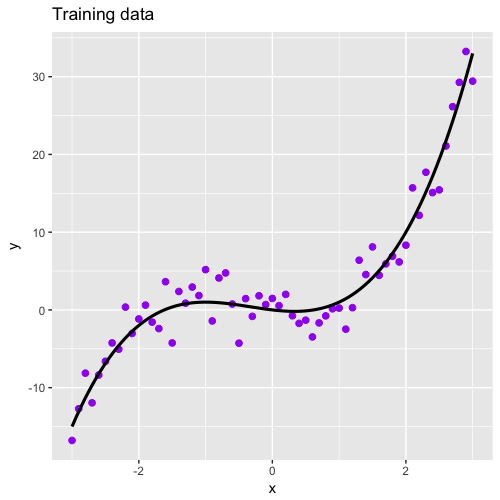
\includegraphics{Prob1f1.png}

In real life we are presented with a data set of pairs \((x_i,y_i)\),
\(i=1,\ldots,n\), and asked to provide a prediction at a value \(x\). We
will use the method of K nearest neighbour regression to do this here.

We have a training set of \(n=61\) observations \((x_i,y_i)\),
\(i=1,\ldots,n\). The KNN regression method provides a prediction at a
value \(x\) by finding the closes \(K\) points and calculating the
average of the observed \(y\) values at these points (Problem 1 at the
2018 TMA4268 exam asked for a precise definition of KNN-regression).

\[\hat{f}(x_0)=\frac{1}{K}\sum_{i\in \mathcal{N}_0} y_i\]

Given an integer \(K\) and a test observation \(x_0\), the KNN
regression first identifies the \(K\) points in the training data that
are closest (Euclidean distance) to \(x_0\), represented by
\(\mathcal{N}_0\). It then estimates the regression curve at \(x_0\) as
the average of the response values for the training observations in
\(\mathcal{N}_0\).

In addition we have a test set of \(n=61\) observations (at the same
grid points as for the training set), but now with new observed values
\(y\).

We have considered \(K=1,\ldots,25\) in the KNN method. Our experiment
has been repeated \(M=1000\) times (that is, \(M\) versions of training
and test set).

\end{block}

\begin{block}{a) Training and test MSE}

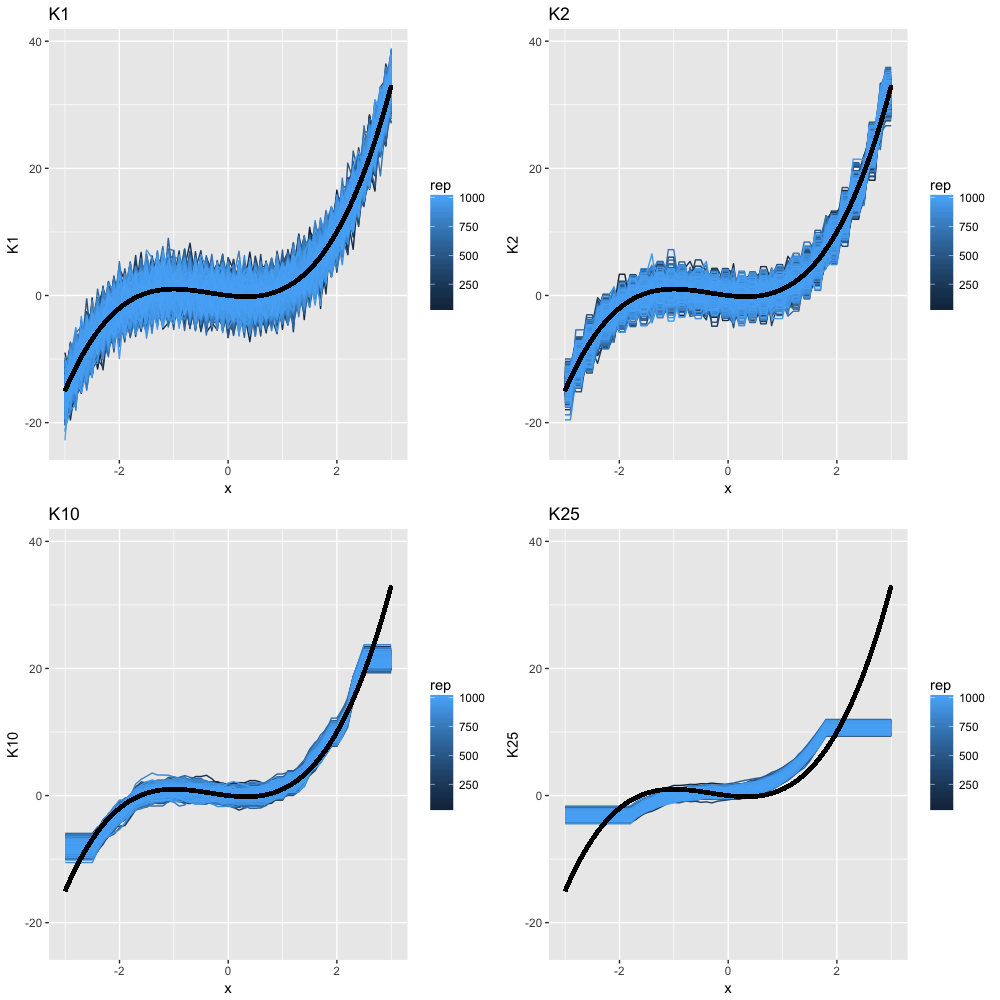
\includegraphics{Prob1f2.png}

In the Figure 2 (above) you see the result of applying the KNN method
with \(K=1,2,10,25\) to our training data, repeated for \(M\) different
training sets (blue lines). The black lines show the true underlying
curve.

\begin{itemize}
\tightlist
\item
  Comment briefly on what you see.
\item
  Does a high or low value of \(K\) give the most flexible fit?
\end{itemize}

In Figure 3 (below) you see mean-squared errors (mean of squared
differences between observed and fitted values) for the training set and
for the test set (right panel for one training and one test set, and
left panel for \(M\)).

\begin{itemize}
\tightlist
\item
  Comment on what you see.
\item
  What do you think is the ``best'' choice for K?
\end{itemize}

Remark: in real life we do not know the true curve, and need to use the
test data to decide on model flexibility (choosing \(K\)).

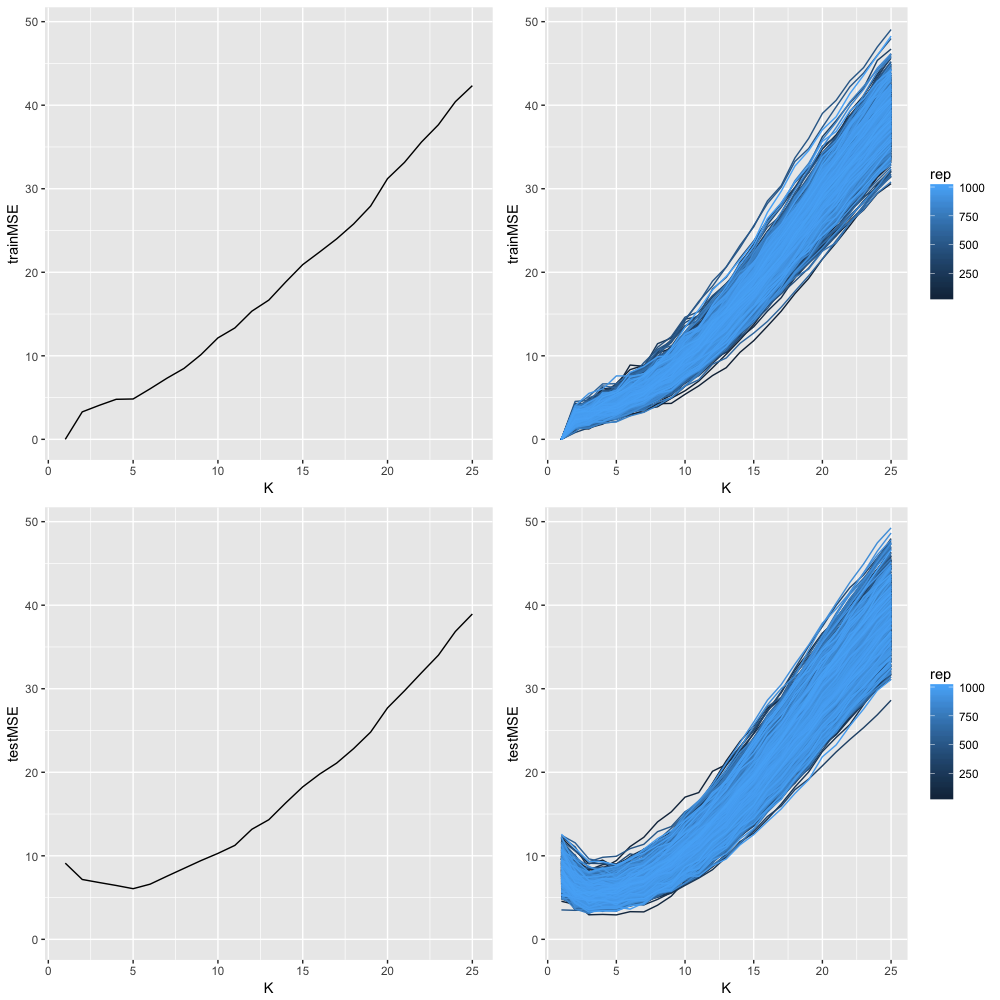
\includegraphics{Prob1f3.png}

\end{block}

\begin{block}{b) Bias-variance trade-off}

Now we leave the real world situation, and assume we know the truth
(this is to focus on bias-variance trade-off). You will not observe
these curves in real life - but the understanding of the bias-variance
trade-off is a core skill in this course!

In the Figure 4 (below) you see a plot of estimated squared bias,
estimated variance, true irreducible error and the sum of these
(labelled total) and averaged over all values of \(x\)

The the squared bias and the variance is calculated based on the
predicted values and the ``true'' values (without the added noise) at
each \(x\).

\begin{itemize}
\tightlist
\item
  Explain how that is done. Hint: this is what the \(M\) repeated
  training data sets are used for.
\item
  Focus on Figure 4. As the flexibility of the model increases (\(K\)
  decreases), what happens with

  \begin{itemize}
  \tightlist
  \item
    the squared bias,\\
  \item
    the variance, and\\
  \item
    the irreducible error?
  \end{itemize}
\item
  What would you recommend is the optimal value of \(K\)? Is this in
  agreement with what you found in a)?
\end{itemize}

Extra: We have chosen to also plot curves at four values of \(x\) -
Figure 5 (below). Based on these four curves, that would you recommend
is the optimal value of \(K\)? Is this in agreement with what you found
previously (averaged over \(x\))?

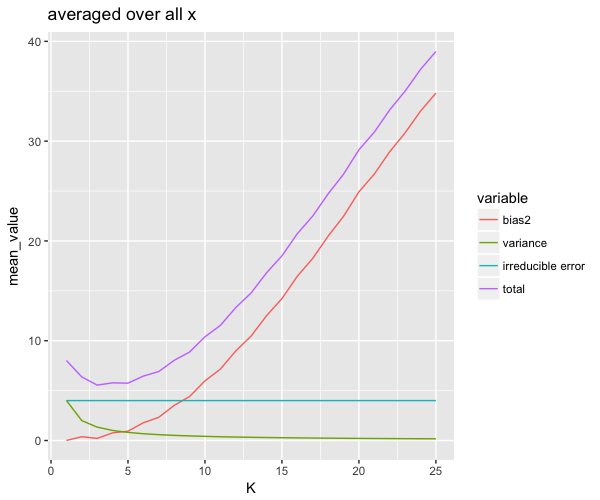
\includegraphics{Prob1f4.png}

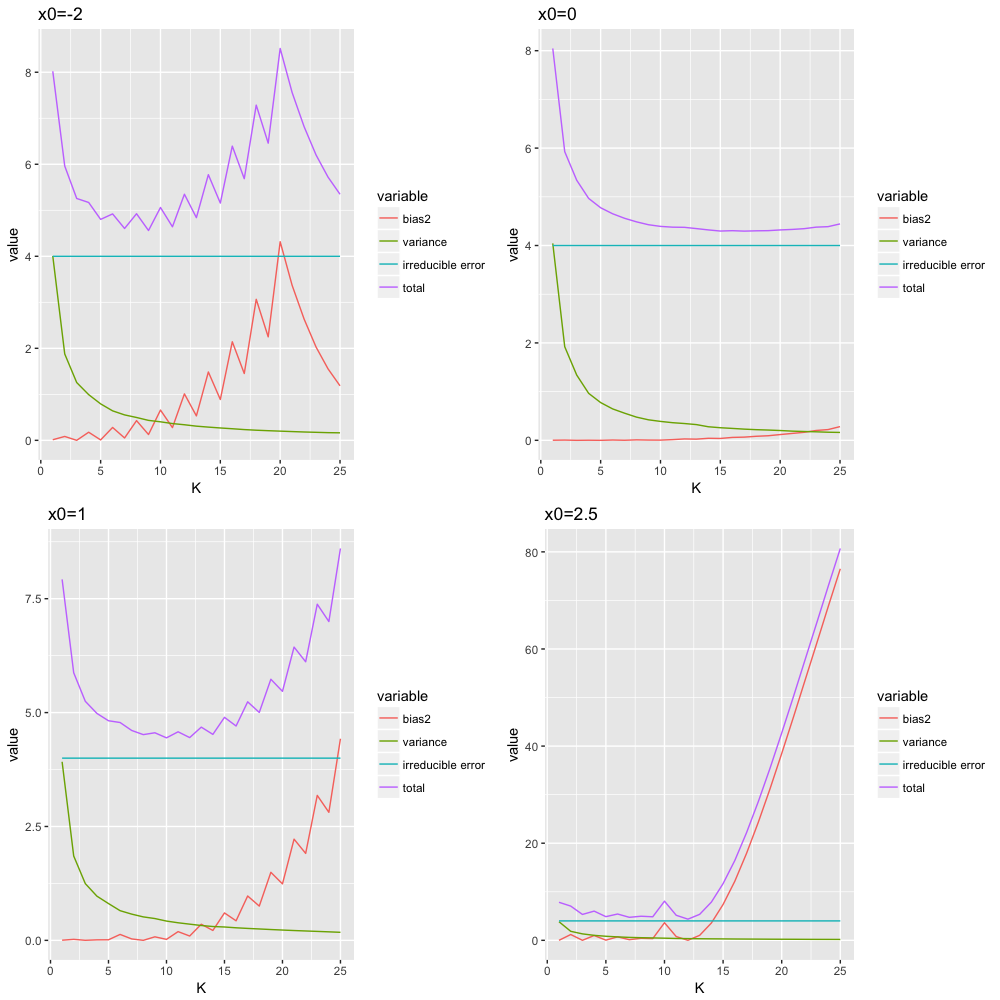
\includegraphics{Prob1f5.png}

\end{block}

\end{frame}

\begin{frame}[fragile]

For completeness the R code used is given next (listed here with
\texttt{M=100} but \texttt{M=1000} was used). You do not need to run the
code, this is just if you have questions about how this was done.

\footnotesize

\begin{Shaded}
\begin{Highlighting}[]
\KeywordTok{library}\NormalTok{(FNN)}
\KeywordTok{library}\NormalTok{(ggplot2)}
\KeywordTok{library}\NormalTok{(ggpubr)}
\KeywordTok{library}\NormalTok{(reshape2)}
\KeywordTok{library}\NormalTok{(dplyr)}
\NormalTok{maxK =}\StringTok{ }\DecValTok{25}
\NormalTok{M =}\StringTok{ }\DecValTok{1000}  \CommentTok{# repeated samplings, x fixed  - examples were run with M=1000}
\NormalTok{x =}\StringTok{ }\KeywordTok{seq}\NormalTok{(}\OperatorTok{-}\DecValTok{3}\NormalTok{, }\DecValTok{3}\NormalTok{, }\FloatTok{0.1}\NormalTok{)}
\NormalTok{dfx =}\StringTok{ }\KeywordTok{data.frame}\NormalTok{(}\DataTypeTok{x =}\NormalTok{ x)}
\NormalTok{truefunc =}\StringTok{ }\ControlFlowTok{function}\NormalTok{(x) }\KeywordTok{return}\NormalTok{(}\OperatorTok{-}\NormalTok{x }\OperatorTok{+}\StringTok{ }\NormalTok{x}\OperatorTok{^}\DecValTok{2} \OperatorTok{+}\StringTok{ }\NormalTok{x}\OperatorTok{^}\DecValTok{3}\NormalTok{)}
\NormalTok{true_y =}\StringTok{ }\KeywordTok{truefunc}\NormalTok{(x)}

\KeywordTok{set.seed}\NormalTok{(}\DecValTok{2}\NormalTok{)  }\CommentTok{# to reproduce}
\NormalTok{error =}\StringTok{ }\KeywordTok{matrix}\NormalTok{(}\KeywordTok{rnorm}\NormalTok{(}\KeywordTok{length}\NormalTok{(x) }\OperatorTok{*}\StringTok{ }\NormalTok{M, }\DataTypeTok{mean =} \DecValTok{0}\NormalTok{, }\DataTypeTok{sd =} \DecValTok{2}\NormalTok{), }\DataTypeTok{nrow =}\NormalTok{ M, }\DataTypeTok{byrow =} \OtherTok{TRUE}\NormalTok{)}
\NormalTok{testerror =}\StringTok{ }\KeywordTok{matrix}\NormalTok{(}\KeywordTok{rnorm}\NormalTok{(}\KeywordTok{length}\NormalTok{(x) }\OperatorTok{*}\StringTok{ }\NormalTok{M, }\DataTypeTok{mean =} \DecValTok{0}\NormalTok{, }\DataTypeTok{sd =} \DecValTok{2}\NormalTok{), }\DataTypeTok{nrow =}\NormalTok{ M, }
    \DataTypeTok{byrow =} \OtherTok{TRUE}\NormalTok{)}
\NormalTok{ymat =}\StringTok{ }\KeywordTok{matrix}\NormalTok{(}\KeywordTok{rep}\NormalTok{(true_y, M), }\DataTypeTok{byrow =}\NormalTok{ T, }\DataTypeTok{nrow =}\NormalTok{ M) }\OperatorTok{+}\StringTok{ }\NormalTok{error}
\NormalTok{testymat =}\StringTok{ }\KeywordTok{matrix}\NormalTok{(}\KeywordTok{rep}\NormalTok{(true_y, M), }\DataTypeTok{byrow =}\NormalTok{ T, }\DataTypeTok{nrow =}\NormalTok{ M) }\OperatorTok{+}\StringTok{ }\NormalTok{testerror}

\KeywordTok{ggplot}\NormalTok{(}\DataTypeTok{data =} \KeywordTok{data.frame}\NormalTok{(}\DataTypeTok{x =}\NormalTok{ x, }\DataTypeTok{y =}\NormalTok{ ymat[}\DecValTok{1}\NormalTok{, ]), }\KeywordTok{aes}\NormalTok{(x, y)) }\OperatorTok{+}\StringTok{ }\KeywordTok{geom_point}\NormalTok{(}\DataTypeTok{col =} \StringTok{"purple"}\NormalTok{, }
    \DataTypeTok{size =} \DecValTok{2}\NormalTok{) }\OperatorTok{+}\StringTok{ }\KeywordTok{stat_function}\NormalTok{(}\DataTypeTok{fun =}\NormalTok{ truefunc, }\DataTypeTok{lwd =} \FloatTok{1.1}\NormalTok{, }\DataTypeTok{colour =} \StringTok{"black"}\NormalTok{) }\OperatorTok{+}\StringTok{ }
\StringTok{    }\KeywordTok{ggtitle}\NormalTok{(}\StringTok{"Training data"}\NormalTok{)}

\NormalTok{predarray =}\StringTok{ }\KeywordTok{array}\NormalTok{(}\OtherTok{NA}\NormalTok{, }\DataTypeTok{dim =} \KeywordTok{c}\NormalTok{(M, }\KeywordTok{length}\NormalTok{(x), maxK))}
\ControlFlowTok{for}\NormalTok{ (i }\ControlFlowTok{in} \DecValTok{1}\OperatorTok{:}\NormalTok{M) \{}
    \ControlFlowTok{for}\NormalTok{ (j }\ControlFlowTok{in} \DecValTok{1}\OperatorTok{:}\NormalTok{maxK) \{}
\NormalTok{        predarray[i, , j] =}\StringTok{ }\KeywordTok{knn.reg}\NormalTok{(}\DataTypeTok{train =}\NormalTok{ dfx, }\DataTypeTok{test =}\NormalTok{ dfx, }\DataTypeTok{y =} \KeywordTok{c}\NormalTok{(ymat[i, }
\NormalTok{            ]), }\DataTypeTok{k =}\NormalTok{ j)}\OperatorTok{$}\NormalTok{pred}
\NormalTok{    \}}
\NormalTok{\}}
\CommentTok{# first - just plot the fitted values - and add the true curve in}
\CommentTok{# black M curves and choose k=1,2,10,30 in KNN}

\CommentTok{# rearranging to get data frame that is useful}
\NormalTok{thislwd =}\StringTok{ }\FloatTok{1.3}
\NormalTok{stackmat =}\StringTok{ }\OtherTok{NULL}
\ControlFlowTok{for}\NormalTok{ (i }\ControlFlowTok{in} \DecValTok{1}\OperatorTok{:}\NormalTok{M) stackmat =}\StringTok{ }\KeywordTok{rbind}\NormalTok{(stackmat, }\KeywordTok{cbind}\NormalTok{(x, }\KeywordTok{rep}\NormalTok{(i, }\KeywordTok{length}\NormalTok{(x)), }
\NormalTok{    predarray[i, , ]))}
\KeywordTok{colnames}\NormalTok{(stackmat) =}\StringTok{ }\KeywordTok{c}\NormalTok{(}\StringTok{"x"}\NormalTok{, }\StringTok{"rep"}\NormalTok{, }\KeywordTok{paste}\NormalTok{(}\StringTok{"K"}\NormalTok{, }\DecValTok{1}\OperatorTok{:}\NormalTok{maxK, }\DataTypeTok{sep =} \StringTok{""}\NormalTok{))}
\NormalTok{sdf =}\StringTok{ }\KeywordTok{as.data.frame}\NormalTok{(stackmat)}
\NormalTok{yrange =}\StringTok{ }\KeywordTok{range}\NormalTok{(}\KeywordTok{apply}\NormalTok{(sdf, }\DecValTok{2}\NormalTok{, range)[, }\DecValTok{3}\OperatorTok{:}\NormalTok{(maxK }\OperatorTok{+}\StringTok{ }\DecValTok{2}\NormalTok{)])}
\CommentTok{# making the four selected plots}
\NormalTok{p1 =}\StringTok{ }\KeywordTok{ggplot}\NormalTok{(}\DataTypeTok{data =}\NormalTok{ sdf, }\KeywordTok{aes}\NormalTok{(}\DataTypeTok{x =}\NormalTok{ x, }\DataTypeTok{y =}\NormalTok{ K1, }\DataTypeTok{group =}\NormalTok{ rep, }\DataTypeTok{colour =}\NormalTok{ rep)) }\OperatorTok{+}\StringTok{ }
\StringTok{    }\KeywordTok{scale_y_continuous}\NormalTok{(}\DataTypeTok{limits =}\NormalTok{ yrange) }\OperatorTok{+}\StringTok{ }\KeywordTok{geom_line}\NormalTok{()}
\NormalTok{p1 =}\StringTok{ }\NormalTok{p1 }\OperatorTok{+}\StringTok{ }\KeywordTok{stat_function}\NormalTok{(}\DataTypeTok{fun =}\NormalTok{ truefunc, }\DataTypeTok{lwd =}\NormalTok{ thislwd, }\DataTypeTok{colour =} \StringTok{"black"}\NormalTok{) }\OperatorTok{+}\StringTok{ }
\StringTok{    }\KeywordTok{ggtitle}\NormalTok{(}\StringTok{"K1"}\NormalTok{)}
\NormalTok{p2 =}\StringTok{ }\KeywordTok{ggplot}\NormalTok{(}\DataTypeTok{data =}\NormalTok{ sdf, }\KeywordTok{aes}\NormalTok{(}\DataTypeTok{x =}\NormalTok{ x, }\DataTypeTok{y =}\NormalTok{ K2, }\DataTypeTok{group =}\NormalTok{ rep, }\DataTypeTok{colour =}\NormalTok{ rep)) }\OperatorTok{+}\StringTok{ }
\StringTok{    }\KeywordTok{scale_y_continuous}\NormalTok{(}\DataTypeTok{limits =}\NormalTok{ yrange) }\OperatorTok{+}\StringTok{ }\KeywordTok{geom_line}\NormalTok{()}
\NormalTok{p2 =}\StringTok{ }\NormalTok{p2 }\OperatorTok{+}\StringTok{ }\KeywordTok{stat_function}\NormalTok{(}\DataTypeTok{fun =}\NormalTok{ truefunc, }\DataTypeTok{lwd =}\NormalTok{ thislwd, }\DataTypeTok{colour =} \StringTok{"black"}\NormalTok{) }\OperatorTok{+}\StringTok{ }
\StringTok{    }\KeywordTok{ggtitle}\NormalTok{(}\StringTok{"K2"}\NormalTok{)}
\NormalTok{p10 =}\StringTok{ }\KeywordTok{ggplot}\NormalTok{(}\DataTypeTok{data =}\NormalTok{ sdf, }\KeywordTok{aes}\NormalTok{(}\DataTypeTok{x =}\NormalTok{ x, }\DataTypeTok{y =}\NormalTok{ K10, }\DataTypeTok{group =}\NormalTok{ rep, }\DataTypeTok{colour =}\NormalTok{ rep)) }\OperatorTok{+}\StringTok{ }
\StringTok{    }\KeywordTok{scale_y_continuous}\NormalTok{(}\DataTypeTok{limits =}\NormalTok{ yrange) }\OperatorTok{+}\StringTok{ }\KeywordTok{geom_line}\NormalTok{()}
\NormalTok{p10 =}\StringTok{ }\NormalTok{p10 }\OperatorTok{+}\StringTok{ }\KeywordTok{stat_function}\NormalTok{(}\DataTypeTok{fun =}\NormalTok{ truefunc, }\DataTypeTok{lwd =}\NormalTok{ thislwd, }\DataTypeTok{colour =} \StringTok{"black"}\NormalTok{) }\OperatorTok{+}\StringTok{ }
\StringTok{    }\KeywordTok{ggtitle}\NormalTok{(}\StringTok{"K10"}\NormalTok{)}
\NormalTok{p25 =}\StringTok{ }\KeywordTok{ggplot}\NormalTok{(}\DataTypeTok{data =}\NormalTok{ sdf, }\KeywordTok{aes}\NormalTok{(}\DataTypeTok{x =}\NormalTok{ x, }\DataTypeTok{y =}\NormalTok{ K25, }\DataTypeTok{group =}\NormalTok{ rep, }\DataTypeTok{colour =}\NormalTok{ rep)) }\OperatorTok{+}\StringTok{ }
\StringTok{    }\KeywordTok{scale_y_continuous}\NormalTok{(}\DataTypeTok{limits =}\NormalTok{ yrange) }\OperatorTok{+}\StringTok{ }\KeywordTok{geom_line}\NormalTok{()}
\NormalTok{p25 =}\StringTok{ }\NormalTok{p25 }\OperatorTok{+}\StringTok{ }\KeywordTok{stat_function}\NormalTok{(}\DataTypeTok{fun =}\NormalTok{ truefunc, }\DataTypeTok{lwd =}\NormalTok{ thislwd, }\DataTypeTok{colour =} \StringTok{"black"}\NormalTok{) }\OperatorTok{+}\StringTok{ }
\StringTok{    }\KeywordTok{ggtitle}\NormalTok{(}\StringTok{"K30"}\NormalTok{)}
\KeywordTok{ggarrange}\NormalTok{(p1, p2, p10, p25)}

\CommentTok{# calculating trainMSE and testMSE}
\NormalTok{trainMSE =}\StringTok{ }\KeywordTok{matrix}\NormalTok{(}\DataTypeTok{ncol =}\NormalTok{ maxK, }\DataTypeTok{nrow =}\NormalTok{ M)}
\ControlFlowTok{for}\NormalTok{ (i }\ControlFlowTok{in} \DecValTok{1}\OperatorTok{:}\NormalTok{M) trainMSE[i, ] =}\StringTok{ }\KeywordTok{apply}\NormalTok{((predarray[i, , ] }\OperatorTok{-}\StringTok{ }\NormalTok{ymat[i, ])}\OperatorTok{^}\DecValTok{2}\NormalTok{, }
    \DecValTok{2}\NormalTok{, mean)}
\NormalTok{testMSE =}\StringTok{ }\KeywordTok{matrix}\NormalTok{(}\DataTypeTok{ncol =}\NormalTok{ maxK, }\DataTypeTok{nrow =}\NormalTok{ M)}
\ControlFlowTok{for}\NormalTok{ (i }\ControlFlowTok{in} \DecValTok{1}\OperatorTok{:}\NormalTok{M) testMSE[i, ] =}\StringTok{ }\KeywordTok{apply}\NormalTok{((predarray[i, , ] }\OperatorTok{-}\StringTok{ }\NormalTok{testymat[i, ])}\OperatorTok{^}\DecValTok{2}\NormalTok{, }
    \DecValTok{2}\NormalTok{, mean)}
\CommentTok{# rearranging to get data frame that is useful}
\NormalTok{stackmat =}\StringTok{ }\OtherTok{NULL}
\ControlFlowTok{for}\NormalTok{ (i }\ControlFlowTok{in} \DecValTok{1}\OperatorTok{:}\NormalTok{M) stackmat =}\StringTok{ }\KeywordTok{rbind}\NormalTok{(stackmat, }\KeywordTok{cbind}\NormalTok{(}\KeywordTok{rep}\NormalTok{(i, maxK), }\DecValTok{1}\OperatorTok{:}\NormalTok{maxK, }
\NormalTok{    trainMSE[i, ], testMSE[i, ]))}
\KeywordTok{colnames}\NormalTok{(stackmat) =}\StringTok{ }\KeywordTok{c}\NormalTok{(}\StringTok{"rep"}\NormalTok{, }\StringTok{"K"}\NormalTok{, }\StringTok{"trainMSE"}\NormalTok{, }\StringTok{"testMSE"}\NormalTok{)}
\NormalTok{sdf =}\StringTok{ }\KeywordTok{as.data.frame}\NormalTok{(stackmat)}
\NormalTok{yrange =}\StringTok{ }\KeywordTok{range}\NormalTok{(sdf[, }\DecValTok{3}\OperatorTok{:}\DecValTok{4}\NormalTok{])}
\CommentTok{# plotting training and test MSE}
\NormalTok{p1 =}\StringTok{ }\KeywordTok{ggplot}\NormalTok{(}\DataTypeTok{data =}\NormalTok{ sdf[}\DecValTok{1}\OperatorTok{:}\NormalTok{maxK, ], }\KeywordTok{aes}\NormalTok{(}\DataTypeTok{x =}\NormalTok{ K, }\DataTypeTok{y =}\NormalTok{ trainMSE)) }\OperatorTok{+}\StringTok{ }\KeywordTok{scale_y_continuous}\NormalTok{(}\DataTypeTok{limits =}\NormalTok{ yrange) }\OperatorTok{+}\StringTok{ }
\StringTok{    }\KeywordTok{geom_line}\NormalTok{()}
\NormalTok{pall =}\StringTok{ }\KeywordTok{ggplot}\NormalTok{(}\DataTypeTok{data =}\NormalTok{ sdf, }\KeywordTok{aes}\NormalTok{(}\DataTypeTok{x =}\NormalTok{ K, }\DataTypeTok{group =}\NormalTok{ rep, }\DataTypeTok{y =}\NormalTok{ trainMSE, }\DataTypeTok{colour =}\NormalTok{ rep)) }\OperatorTok{+}\StringTok{ }
\StringTok{    }\KeywordTok{scale_y_continuous}\NormalTok{(}\DataTypeTok{limits =}\NormalTok{ yrange) }\OperatorTok{+}\StringTok{ }\KeywordTok{geom_line}\NormalTok{()}
\NormalTok{testp1 =}\StringTok{ }\KeywordTok{ggplot}\NormalTok{(}\DataTypeTok{data =}\NormalTok{ sdf[}\DecValTok{1}\OperatorTok{:}\NormalTok{maxK, ], }\KeywordTok{aes}\NormalTok{(}\DataTypeTok{x =}\NormalTok{ K, }\DataTypeTok{y =}\NormalTok{ testMSE)) }\OperatorTok{+}\StringTok{ }\KeywordTok{scale_y_continuous}\NormalTok{(}\DataTypeTok{limits =}\NormalTok{ yrange) }\OperatorTok{+}\StringTok{ }
\StringTok{    }\KeywordTok{geom_line}\NormalTok{()}
\NormalTok{testpall =}\StringTok{ }\KeywordTok{ggplot}\NormalTok{(}\DataTypeTok{data =}\NormalTok{ sdf, }\KeywordTok{aes}\NormalTok{(}\DataTypeTok{x =}\NormalTok{ K, }\DataTypeTok{group =}\NormalTok{ rep, }\DataTypeTok{y =}\NormalTok{ testMSE, }\DataTypeTok{colour =}\NormalTok{ rep)) }\OperatorTok{+}\StringTok{ }
\StringTok{    }\KeywordTok{scale_y_continuous}\NormalTok{(}\DataTypeTok{limits =}\NormalTok{ yrange) }\OperatorTok{+}\StringTok{ }\KeywordTok{geom_line}\NormalTok{()}
\KeywordTok{ggarrange}\NormalTok{(p1, pall, testp1, testpall)}

\CommentTok{# calculating bias^2 and variance}
\NormalTok{meanmat =}\StringTok{ }\KeywordTok{matrix}\NormalTok{(}\DataTypeTok{ncol =} \KeywordTok{length}\NormalTok{(x), }\DataTypeTok{nrow =}\NormalTok{ maxK)}
\NormalTok{varmat =}\StringTok{ }\KeywordTok{matrix}\NormalTok{(}\DataTypeTok{ncol =} \KeywordTok{length}\NormalTok{(x), }\DataTypeTok{nrow =}\NormalTok{ maxK)}
\ControlFlowTok{for}\NormalTok{ (j }\ControlFlowTok{in} \DecValTok{1}\OperatorTok{:}\NormalTok{maxK) \{}
\NormalTok{    meanmat[j, ] =}\StringTok{ }\KeywordTok{apply}\NormalTok{(predarray[, , j], }\DecValTok{2}\NormalTok{, mean)  }\CommentTok{# we now take the mean over the M simulations - to mimic E and Var at each x value and each KNN model}
\NormalTok{    varmat[j, ] =}\StringTok{ }\KeywordTok{apply}\NormalTok{(predarray[, , j], }\DecValTok{2}\NormalTok{, var)}
\NormalTok{\}}
\NormalTok{bias2mat =}\StringTok{ }\NormalTok{(meanmat }\OperatorTok{-}\StringTok{ }\KeywordTok{matrix}\NormalTok{(}\KeywordTok{rep}\NormalTok{(true_y, maxK), }\DataTypeTok{byrow =} \OtherTok{TRUE}\NormalTok{, }\DataTypeTok{nrow =}\NormalTok{ maxK))}\OperatorTok{^}\DecValTok{2}  \CommentTok{#here the truth is finally used!}

\CommentTok{# preparing to plot}
\NormalTok{df =}\StringTok{ }\KeywordTok{data.frame}\NormalTok{(}\KeywordTok{rep}\NormalTok{(x, }\DataTypeTok{each =}\NormalTok{ maxK), }\KeywordTok{rep}\NormalTok{(}\DecValTok{1}\OperatorTok{:}\NormalTok{maxK, }\KeywordTok{length}\NormalTok{(x)), }\KeywordTok{c}\NormalTok{(bias2mat), }
    \KeywordTok{c}\NormalTok{(varmat), }\KeywordTok{rep}\NormalTok{(}\DecValTok{4}\NormalTok{, }\KeywordTok{prod}\NormalTok{(}\KeywordTok{dim}\NormalTok{(varmat))))  }\CommentTok{#irr is just 4}
\KeywordTok{colnames}\NormalTok{(df) =}\StringTok{ }\KeywordTok{c}\NormalTok{(}\StringTok{"x"}\NormalTok{, }\StringTok{"K"}\NormalTok{, }\StringTok{"bias2"}\NormalTok{, }\StringTok{"variance"}\NormalTok{, }\StringTok{"irreducible error"}\NormalTok{)  }\CommentTok{#suitable for plotting}
\NormalTok{df}\OperatorTok{$}\NormalTok{total =}\StringTok{ }\NormalTok{df}\OperatorTok{$}\NormalTok{bias2 }\OperatorTok{+}\StringTok{ }\NormalTok{df}\OperatorTok{$}\NormalTok{variance }\OperatorTok{+}\StringTok{ }\NormalTok{df}\OperatorTok{$}\StringTok{`}\DataTypeTok{irreducible error}\StringTok{`}
\NormalTok{hdf =}\StringTok{ }\KeywordTok{melt}\NormalTok{(df, }\DataTypeTok{id =} \KeywordTok{c}\NormalTok{(}\StringTok{"x"}\NormalTok{, }\StringTok{"K"}\NormalTok{))}
\CommentTok{# averaged over all x - to compare to train and test MSE}
\NormalTok{hdfmean =}\StringTok{ }\NormalTok{hdf }\OperatorTok\StringTok{ }\KeywordTok{group_by}\NormalTok{(K, variable) }\OperatorTok\StringTok{ }\KeywordTok{summarise}\NormalTok{(}\DataTypeTok{mean_value =} \KeywordTok{mean}\NormalTok{(value))}
\KeywordTok{ggplot}\NormalTok{(}\DataTypeTok{data =}\NormalTok{ hdfmean[hdfmean[, }\DecValTok{1}\NormalTok{] }\OperatorTok{<}\StringTok{ }\DecValTok{31}\NormalTok{, ], }\KeywordTok{aes}\NormalTok{(}\DataTypeTok{x =}\NormalTok{ K, }\DataTypeTok{y =}\NormalTok{ mean_value, }
    \DataTypeTok{colour =}\NormalTok{ variable)) }\OperatorTok{+}\StringTok{ }\KeywordTok{geom_line}\NormalTok{() }\OperatorTok{+}\StringTok{ }\KeywordTok{ggtitle}\NormalTok{(}\StringTok{"averaged over all x"}\NormalTok{)}

\CommentTok{# extra: what about different values of x?}
\NormalTok{hdfatxa =}\StringTok{ }\NormalTok{hdf[hdf}\OperatorTok{$}\NormalTok{x }\OperatorTok{==}\StringTok{ }\DecValTok{-2}\NormalTok{, ]}
\NormalTok{hdfatxb =}\StringTok{ }\NormalTok{hdf[hdf}\OperatorTok{$}\NormalTok{x }\OperatorTok{==}\StringTok{ }\DecValTok{0}\NormalTok{, ]}
\NormalTok{hdfatxc =}\StringTok{ }\NormalTok{hdf[hdf}\OperatorTok{$}\NormalTok{x }\OperatorTok{==}\StringTok{ }\DecValTok{1}\NormalTok{, ]}
\NormalTok{hdfatxd =}\StringTok{ }\NormalTok{hdf[hdf}\OperatorTok{$}\NormalTok{x }\OperatorTok{==}\StringTok{ }\FloatTok{2.5}\NormalTok{, ]}
\NormalTok{pa =}\StringTok{ }\KeywordTok{ggplot}\NormalTok{(}\DataTypeTok{data =}\NormalTok{ hdfatxa, }\KeywordTok{aes}\NormalTok{(}\DataTypeTok{x =}\NormalTok{ K, }\DataTypeTok{y =}\NormalTok{ value, }\DataTypeTok{colour =}\NormalTok{ variable)) }\OperatorTok{+}\StringTok{ }
\StringTok{    }\KeywordTok{geom_line}\NormalTok{() }\OperatorTok{+}\StringTok{ }\KeywordTok{ggtitle}\NormalTok{(}\StringTok{"x0=-2"}\NormalTok{)}
\NormalTok{pb =}\StringTok{ }\KeywordTok{ggplot}\NormalTok{(}\DataTypeTok{data =}\NormalTok{ hdfatxb, }\KeywordTok{aes}\NormalTok{(}\DataTypeTok{x =}\NormalTok{ K, }\DataTypeTok{y =}\NormalTok{ value, }\DataTypeTok{colour =}\NormalTok{ variable)) }\OperatorTok{+}\StringTok{ }
\StringTok{    }\KeywordTok{geom_line}\NormalTok{() }\OperatorTok{+}\StringTok{ }\KeywordTok{ggtitle}\NormalTok{(}\StringTok{"x0=0"}\NormalTok{)}
\NormalTok{pc =}\StringTok{ }\KeywordTok{ggplot}\NormalTok{(}\DataTypeTok{data =}\NormalTok{ hdfatxc, }\KeywordTok{aes}\NormalTok{(}\DataTypeTok{x =}\NormalTok{ K, }\DataTypeTok{y =}\NormalTok{ value, }\DataTypeTok{colour =}\NormalTok{ variable)) }\OperatorTok{+}\StringTok{ }
\StringTok{    }\KeywordTok{geom_line}\NormalTok{() }\OperatorTok{+}\StringTok{ }\KeywordTok{ggtitle}\NormalTok{(}\StringTok{"x0=1"}\NormalTok{)}
\NormalTok{pd =}\StringTok{ }\KeywordTok{ggplot}\NormalTok{(}\DataTypeTok{data =}\NormalTok{ hdfatxd, }\KeywordTok{aes}\NormalTok{(}\DataTypeTok{x =}\NormalTok{ K, }\DataTypeTok{y =}\NormalTok{ value, }\DataTypeTok{colour =}\NormalTok{ variable)) }\OperatorTok{+}\StringTok{ }
\StringTok{    }\KeywordTok{geom_line}\NormalTok{() }\OperatorTok{+}\StringTok{ }\KeywordTok{ggtitle}\NormalTok{(}\StringTok{"x0=2.5"}\NormalTok{)}
\KeywordTok{ggarrange}\NormalTok{(pa, pb, pc, pd)}
\end{Highlighting}
\end{Shaded}

\normalsize

\begin{block}{Problem 3: Theory and practice - MSEtrain, MSEtest, and
bias-variance}

We will now look closely into the simulations and calculations performed
for the MSEtrain, MSEtest, and bias-variance trade-off in PartA.

\begin{itemize}
\tightlist
\item
  The simulations are based on \(f(x)=x^2\) and normal noise with mean 0
  and standard deviation 2 is added.
\item
  \(x\) is on a 0.1 grid from -2 to 4 (61 values).
\item
  Parametric models of different complexity are fitted - poly1-poly20.
\item
  M=100 simulations are done.
\end{itemize}

The aim of this problem is to understand:

\begin{itemize}
\tightlist
\item
  trainMSE
\item
  testMSE
\item
  bias-variance trade-off
\end{itemize}

\end{block}

\end{frame}

\begin{frame}[fragile]

\begin{block}{a) Problem set-up}

\begin{itemize}
\tightlist
\item
  See the code below. Explain what is done. (You need not understand the
  code in detail.) Run the code.
\item
  We will learn more about the \texttt{lm} function in M 3 - now just
  think of this as fitting a polynomial regression and predict gives the
  fitted curve in our grid points. \texttt{predarray} is just a way to
  save M simulations of 61 gridpoints in x and 20 polynomial models.
\end{itemize}

\begin{Shaded}
\begin{Highlighting}[]
\KeywordTok{library}\NormalTok{(ggplot2)}
\KeywordTok{library}\NormalTok{(ggpubr)}
\KeywordTok{set.seed}\NormalTok{(}\DecValTok{2}\NormalTok{)  }\CommentTok{# to reproduce}

\NormalTok{M =}\StringTok{ }\DecValTok{100}  \CommentTok{# repeated samplings, x fixed }
\NormalTok{nord =}\StringTok{ }\DecValTok{20}  \CommentTok{# order of polynoms}


\NormalTok{x =}\StringTok{ }\KeywordTok{seq}\NormalTok{(}\OperatorTok{-}\DecValTok{2}\NormalTok{, }\DecValTok{4}\NormalTok{, }\FloatTok{0.1}\NormalTok{)}
\NormalTok{truefunc =}\StringTok{ }\ControlFlowTok{function}\NormalTok{(x) }\KeywordTok{return}\NormalTok{(x}\OperatorTok{^}\DecValTok{2}\NormalTok{)}
\NormalTok{true_y =}\StringTok{ }\KeywordTok{truefunc}\NormalTok{(x)}

\NormalTok{error =}\StringTok{ }\KeywordTok{matrix}\NormalTok{(}\KeywordTok{rnorm}\NormalTok{(}\KeywordTok{length}\NormalTok{(x) }\OperatorTok{*}\StringTok{ }\NormalTok{M, }\DataTypeTok{mean =} \DecValTok{0}\NormalTok{, }\DataTypeTok{sd =} \DecValTok{2}\NormalTok{), }\DataTypeTok{nrow =}\NormalTok{ M, }\DataTypeTok{byrow =} \OtherTok{TRUE}\NormalTok{)}
\NormalTok{ymat =}\StringTok{ }\KeywordTok{matrix}\NormalTok{(}\KeywordTok{rep}\NormalTok{(true_y, M), }\DataTypeTok{byrow =}\NormalTok{ T, }\DataTypeTok{nrow =}\NormalTok{ M) }\OperatorTok{+}\StringTok{ }\NormalTok{error}

\NormalTok{predarray =}\StringTok{ }\KeywordTok{array}\NormalTok{(}\OtherTok{NA}\NormalTok{, }\DataTypeTok{dim =} \KeywordTok{c}\NormalTok{(M, }\KeywordTok{length}\NormalTok{(x), nord))}
\ControlFlowTok{for}\NormalTok{ (i }\ControlFlowTok{in} \DecValTok{1}\OperatorTok{:}\NormalTok{M) \{}
    \ControlFlowTok{for}\NormalTok{ (j }\ControlFlowTok{in} \DecValTok{1}\OperatorTok{:}\NormalTok{nord) \{}
\NormalTok{        predarray[i, , j] =}\StringTok{ }\KeywordTok{predict}\NormalTok{(}\KeywordTok{lm}\NormalTok{(ymat[i, ] }\OperatorTok{~}\StringTok{ }\KeywordTok{poly}\NormalTok{(x, j, }\DataTypeTok{raw =} \OtherTok{TRUE}\NormalTok{)))}
\NormalTok{    \}}
\NormalTok{\}}
\CommentTok{# M matrices of size length(x) times nord first, only look at}
\CommentTok{# variablity in the M fits and plot M curves where we had 1}

\CommentTok{# for plotting need to stack the matrices underneath eachother and}
\CommentTok{# make new variable 'rep'}
\NormalTok{stackmat =}\StringTok{ }\OtherTok{NULL}
\ControlFlowTok{for}\NormalTok{ (i }\ControlFlowTok{in} \DecValTok{1}\OperatorTok{:}\NormalTok{M) stackmat =}\StringTok{ }\KeywordTok{rbind}\NormalTok{(stackmat, }\KeywordTok{cbind}\NormalTok{(x, }\KeywordTok{rep}\NormalTok{(i, }\KeywordTok{length}\NormalTok{(x)), }
\NormalTok{    predarray[i, , ]))}
\CommentTok{# dim(stackmat)}
\KeywordTok{colnames}\NormalTok{(stackmat) =}\StringTok{ }\KeywordTok{c}\NormalTok{(}\StringTok{"x"}\NormalTok{, }\StringTok{"rep"}\NormalTok{, }\KeywordTok{paste}\NormalTok{(}\StringTok{"poly"}\NormalTok{, }\DecValTok{1}\OperatorTok{:}\DecValTok{20}\NormalTok{, }\DataTypeTok{sep =} \StringTok{""}\NormalTok{))}
\NormalTok{sdf =}\StringTok{ }\KeywordTok{as.data.frame}\NormalTok{(stackmat)  }\CommentTok{#NB have poly1-20 now - but first only use 1,2,20}
\CommentTok{# to add true curve using stat_function - easiest solution}
\NormalTok{true_x =}\StringTok{ }\NormalTok{x}
\NormalTok{yrange =}\StringTok{ }\KeywordTok{range}\NormalTok{(}\KeywordTok{apply}\NormalTok{(sdf, }\DecValTok{2}\NormalTok{, range)[, }\DecValTok{3}\OperatorTok{:}\DecValTok{22}\NormalTok{])}
\NormalTok{p1 =}\StringTok{ }\KeywordTok{ggplot}\NormalTok{(}\DataTypeTok{data =}\NormalTok{ sdf, }\KeywordTok{aes}\NormalTok{(}\DataTypeTok{x =}\NormalTok{ x, }\DataTypeTok{y =}\NormalTok{ poly1, }\DataTypeTok{group =}\NormalTok{ rep, }\DataTypeTok{colour =}\NormalTok{ rep)) }\OperatorTok{+}\StringTok{ }
\StringTok{    }\KeywordTok{scale_y_continuous}\NormalTok{(}\DataTypeTok{limits =}\NormalTok{ yrange) }\OperatorTok{+}\StringTok{ }\KeywordTok{geom_line}\NormalTok{()}
\NormalTok{p1 =}\StringTok{ }\NormalTok{p1 }\OperatorTok{+}\StringTok{ }\KeywordTok{stat_function}\NormalTok{(}\DataTypeTok{fun =}\NormalTok{ truefunc, }\DataTypeTok{lwd =} \FloatTok{1.3}\NormalTok{, }\DataTypeTok{colour =} \StringTok{"black"}\NormalTok{) }\OperatorTok{+}\StringTok{ }
\StringTok{    }\KeywordTok{ggtitle}\NormalTok{(}\StringTok{"poly1"}\NormalTok{)}
\NormalTok{p2 =}\StringTok{ }\KeywordTok{ggplot}\NormalTok{(}\DataTypeTok{data =}\NormalTok{ sdf, }\KeywordTok{aes}\NormalTok{(}\DataTypeTok{x =}\NormalTok{ x, }\DataTypeTok{y =}\NormalTok{ poly2, }\DataTypeTok{group =}\NormalTok{ rep, }\DataTypeTok{colour =}\NormalTok{ rep)) }\OperatorTok{+}\StringTok{ }
\StringTok{    }\KeywordTok{scale_y_continuous}\NormalTok{(}\DataTypeTok{limits =}\NormalTok{ yrange) }\OperatorTok{+}\StringTok{ }\KeywordTok{geom_line}\NormalTok{()}
\NormalTok{p2 =}\StringTok{ }\NormalTok{p2 }\OperatorTok{+}\StringTok{ }\KeywordTok{stat_function}\NormalTok{(}\DataTypeTok{fun =}\NormalTok{ truefunc, }\DataTypeTok{lwd =} \FloatTok{1.3}\NormalTok{, }\DataTypeTok{colour =} \StringTok{"black"}\NormalTok{) }\OperatorTok{+}\StringTok{ }
\StringTok{    }\KeywordTok{ggtitle}\NormalTok{(}\StringTok{"poly2"}\NormalTok{)}
\NormalTok{p10 =}\StringTok{ }\KeywordTok{ggplot}\NormalTok{(}\DataTypeTok{data =}\NormalTok{ sdf, }\KeywordTok{aes}\NormalTok{(}\DataTypeTok{x =}\NormalTok{ x, }\DataTypeTok{y =}\NormalTok{ poly10, }\DataTypeTok{group =}\NormalTok{ rep, }\DataTypeTok{colour =}\NormalTok{ rep)) }\OperatorTok{+}\StringTok{ }
\StringTok{    }\KeywordTok{scale_y_continuous}\NormalTok{(}\DataTypeTok{limits =}\NormalTok{ yrange) }\OperatorTok{+}\StringTok{ }\KeywordTok{geom_line}\NormalTok{()}
\NormalTok{p10 =}\StringTok{ }\NormalTok{p10 }\OperatorTok{+}\StringTok{ }\KeywordTok{stat_function}\NormalTok{(}\DataTypeTok{fun =}\NormalTok{ truefunc, }\DataTypeTok{lwd =} \FloatTok{1.3}\NormalTok{, }\DataTypeTok{colour =} \StringTok{"black"}\NormalTok{) }\OperatorTok{+}\StringTok{ }
\StringTok{    }\KeywordTok{ggtitle}\NormalTok{(}\StringTok{"poly10"}\NormalTok{)}
\NormalTok{p20 =}\StringTok{ }\KeywordTok{ggplot}\NormalTok{(}\DataTypeTok{data =}\NormalTok{ sdf, }\KeywordTok{aes}\NormalTok{(}\DataTypeTok{x =}\NormalTok{ x, }\DataTypeTok{y =}\NormalTok{ poly20, }\DataTypeTok{group =}\NormalTok{ rep, }\DataTypeTok{colour =}\NormalTok{ rep)) }\OperatorTok{+}\StringTok{ }
\StringTok{    }\KeywordTok{scale_y_continuous}\NormalTok{(}\DataTypeTok{limits =}\NormalTok{ yrange) }\OperatorTok{+}\StringTok{ }\KeywordTok{geom_line}\NormalTok{()}
\NormalTok{p20 =}\StringTok{ }\NormalTok{p20 }\OperatorTok{+}\StringTok{ }\KeywordTok{stat_function}\NormalTok{(}\DataTypeTok{fun =}\NormalTok{ truefunc, }\DataTypeTok{lwd =} \FloatTok{1.3}\NormalTok{, }\DataTypeTok{colour =} \StringTok{"black"}\NormalTok{) }\OperatorTok{+}\StringTok{ }
\StringTok{    }\KeywordTok{ggtitle}\NormalTok{(}\StringTok{"poly20"}\NormalTok{)}
\KeywordTok{ggarrange}\NormalTok{(p1, p2, p10, p20)}
\end{Highlighting}
\end{Shaded}

\end{block}

\end{frame}

\begin{frame}[fragile]

\begin{block}{b) Train and test MSE}

\begin{itemize}
\tightlist
\item
  First we produce predictions at each grid point based on our training
  data (\texttt{x} and \texttt{ymat})
\item
  but we also draw new observations to calculate testMSE - see
  \texttt{testymat}
\item
  observe how trainMSE and testMSE is calculated
\item
  run the code
\end{itemize}

\begin{Shaded}
\begin{Highlighting}[]
\KeywordTok{set.seed}\NormalTok{(}\DecValTok{2}\NormalTok{)  }\CommentTok{# to reproduce}

\NormalTok{M =}\StringTok{ }\DecValTok{100}  \CommentTok{# repeated samplings,x fixed but new errors}
\NormalTok{nord =}\StringTok{ }\DecValTok{20}
\NormalTok{x =}\StringTok{ }\KeywordTok{seq}\NormalTok{(}\OperatorTok{-}\DecValTok{2}\NormalTok{, }\DecValTok{4}\NormalTok{, }\FloatTok{0.1}\NormalTok{)}
\NormalTok{truefunc =}\StringTok{ }\ControlFlowTok{function}\NormalTok{(x) }\KeywordTok{return}\NormalTok{(x}\OperatorTok{^}\DecValTok{2}\NormalTok{)}
\NormalTok{true_y =}\StringTok{ }\KeywordTok{truefunc}\NormalTok{(x)}

\NormalTok{error =}\StringTok{ }\KeywordTok{matrix}\NormalTok{(}\KeywordTok{rnorm}\NormalTok{(}\KeywordTok{length}\NormalTok{(x) }\OperatorTok{*}\StringTok{ }\NormalTok{M, }\DataTypeTok{mean =} \DecValTok{0}\NormalTok{, }\DataTypeTok{sd =} \DecValTok{2}\NormalTok{), }\DataTypeTok{nrow =}\NormalTok{ M, }\DataTypeTok{byrow =} \OtherTok{TRUE}\NormalTok{)}
\NormalTok{testerror =}\StringTok{ }\KeywordTok{matrix}\NormalTok{(}\KeywordTok{rnorm}\NormalTok{(}\KeywordTok{length}\NormalTok{(x) }\OperatorTok{*}\StringTok{ }\NormalTok{M, }\DataTypeTok{mean =} \DecValTok{0}\NormalTok{, }\DataTypeTok{sd =} \DecValTok{2}\NormalTok{), }\DataTypeTok{nrow =}\NormalTok{ M, }
    \DataTypeTok{byrow =} \OtherTok{TRUE}\NormalTok{)}
\NormalTok{ymat =}\StringTok{ }\KeywordTok{matrix}\NormalTok{(}\KeywordTok{rep}\NormalTok{(true_y, M), }\DataTypeTok{byrow =}\NormalTok{ T, }\DataTypeTok{nrow =}\NormalTok{ M) }\OperatorTok{+}\StringTok{ }\NormalTok{error}
\NormalTok{testymat =}\StringTok{ }\KeywordTok{matrix}\NormalTok{(}\KeywordTok{rep}\NormalTok{(true_y, M), }\DataTypeTok{byrow =}\NormalTok{ T, }\DataTypeTok{nrow =}\NormalTok{ M) }\OperatorTok{+}\StringTok{ }\NormalTok{testerror}

\NormalTok{predarray =}\StringTok{ }\KeywordTok{array}\NormalTok{(}\OtherTok{NA}\NormalTok{, }\DataTypeTok{dim =} \KeywordTok{c}\NormalTok{(M, }\KeywordTok{length}\NormalTok{(x), nord))}
\ControlFlowTok{for}\NormalTok{ (i }\ControlFlowTok{in} \DecValTok{1}\OperatorTok{:}\NormalTok{M) \{}
    \ControlFlowTok{for}\NormalTok{ (j }\ControlFlowTok{in} \DecValTok{1}\OperatorTok{:}\NormalTok{nord) \{}
\NormalTok{        predarray[i, , j] =}\StringTok{ }\KeywordTok{predict}\NormalTok{(}\KeywordTok{lm}\NormalTok{(ymat[i, ] }\OperatorTok{~}\StringTok{ }\KeywordTok{poly}\NormalTok{(x, j, }\DataTypeTok{raw =} \OtherTok{TRUE}\NormalTok{)))}
\NormalTok{    \}}
\NormalTok{\}}
\NormalTok{trainMSE =}\StringTok{ }\KeywordTok{matrix}\NormalTok{(}\DataTypeTok{ncol =}\NormalTok{ nord, }\DataTypeTok{nrow =}\NormalTok{ M)}
\ControlFlowTok{for}\NormalTok{ (i }\ControlFlowTok{in} \DecValTok{1}\OperatorTok{:}\NormalTok{M) trainMSE[i, ] =}\StringTok{ }\KeywordTok{apply}\NormalTok{((predarray[i, , ] }\OperatorTok{-}\StringTok{ }\NormalTok{ymat[i, ])}\OperatorTok{^}\DecValTok{2}\NormalTok{, }
    \DecValTok{2}\NormalTok{, mean)}
\NormalTok{testMSE =}\StringTok{ }\KeywordTok{matrix}\NormalTok{(}\DataTypeTok{ncol =}\NormalTok{ nord, }\DataTypeTok{nrow =}\NormalTok{ M)}
\ControlFlowTok{for}\NormalTok{ (i }\ControlFlowTok{in} \DecValTok{1}\OperatorTok{:}\NormalTok{M) testMSE[i, ] =}\StringTok{ }\KeywordTok{apply}\NormalTok{((predarray[i, , ] }\OperatorTok{-}\StringTok{ }\NormalTok{testymat[i, ])}\OperatorTok{^}\DecValTok{2}\NormalTok{, }
    \DecValTok{2}\NormalTok{, mean)}
\end{Highlighting}
\end{Shaded}

\begin{itemize}
\tightlist
\item
  Then we plot train and testMSE - first for one train + test data set,
  then for 99 more.
\end{itemize}

\begin{Shaded}
\begin{Highlighting}[]
\KeywordTok{library}\NormalTok{(ggplot2)}
\KeywordTok{library}\NormalTok{(ggpubr)}

\CommentTok{# format suitable for plotting}
\NormalTok{stackmat =}\StringTok{ }\OtherTok{NULL}
\ControlFlowTok{for}\NormalTok{ (i }\ControlFlowTok{in} \DecValTok{1}\OperatorTok{:}\NormalTok{M) stackmat =}\StringTok{ }\KeywordTok{rbind}\NormalTok{(stackmat, }\KeywordTok{cbind}\NormalTok{(}\KeywordTok{rep}\NormalTok{(i, nord), }\DecValTok{1}\OperatorTok{:}\NormalTok{nord, }
\NormalTok{    trainMSE[i, ], testMSE[i, ]))}
\KeywordTok{colnames}\NormalTok{(stackmat) =}\StringTok{ }\KeywordTok{c}\NormalTok{(}\StringTok{"rep"}\NormalTok{, }\StringTok{"poly"}\NormalTok{, }\StringTok{"trainMSE"}\NormalTok{, }\StringTok{"testMSE"}\NormalTok{)}
\NormalTok{sdf =}\StringTok{ }\KeywordTok{as.data.frame}\NormalTok{(stackmat)}
\NormalTok{yrange =}\StringTok{ }\KeywordTok{range}\NormalTok{(sdf[, }\DecValTok{3}\OperatorTok{:}\DecValTok{4}\NormalTok{])}
\NormalTok{p1 =}\StringTok{ }\KeywordTok{ggplot}\NormalTok{(}\DataTypeTok{data =}\NormalTok{ sdf[}\DecValTok{1}\OperatorTok{:}\NormalTok{nord, ], }\KeywordTok{aes}\NormalTok{(}\DataTypeTok{x =}\NormalTok{ poly, }\DataTypeTok{y =}\NormalTok{ trainMSE)) }\OperatorTok{+}\StringTok{ }\KeywordTok{scale_y_continuous}\NormalTok{(}\DataTypeTok{limits =}\NormalTok{ yrange) }\OperatorTok{+}\StringTok{ }
\StringTok{    }\KeywordTok{geom_line}\NormalTok{()}
\NormalTok{pall =}\StringTok{ }\KeywordTok{ggplot}\NormalTok{(}\DataTypeTok{data =}\NormalTok{ sdf, }\KeywordTok{aes}\NormalTok{(}\DataTypeTok{x =}\NormalTok{ poly, }\DataTypeTok{group =}\NormalTok{ rep, }\DataTypeTok{y =}\NormalTok{ trainMSE, }\DataTypeTok{colour =}\NormalTok{ rep)) }\OperatorTok{+}\StringTok{ }
\StringTok{    }\KeywordTok{scale_y_continuous}\NormalTok{(}\DataTypeTok{limits =}\NormalTok{ yrange) }\OperatorTok{+}\StringTok{ }\KeywordTok{geom_line}\NormalTok{()}
\NormalTok{testp1 =}\StringTok{ }\KeywordTok{ggplot}\NormalTok{(}\DataTypeTok{data =}\NormalTok{ sdf[}\DecValTok{1}\OperatorTok{:}\NormalTok{nord, ], }\KeywordTok{aes}\NormalTok{(}\DataTypeTok{x =}\NormalTok{ poly, }\DataTypeTok{y =}\NormalTok{ testMSE)) }\OperatorTok{+}\StringTok{ }\KeywordTok{scale_y_continuous}\NormalTok{(}\DataTypeTok{limits =}\NormalTok{ yrange) }\OperatorTok{+}\StringTok{ }
\StringTok{    }\KeywordTok{geom_line}\NormalTok{()}
\NormalTok{testpall =}\StringTok{ }\KeywordTok{ggplot}\NormalTok{(}\DataTypeTok{data =}\NormalTok{ sdf, }\KeywordTok{aes}\NormalTok{(}\DataTypeTok{x =}\NormalTok{ poly, }\DataTypeTok{group =}\NormalTok{ rep, }\DataTypeTok{y =}\NormalTok{ testMSE, }
    \DataTypeTok{colour =}\NormalTok{ rep)) }\OperatorTok{+}\StringTok{ }\KeywordTok{scale_y_continuous}\NormalTok{(}\DataTypeTok{limits =}\NormalTok{ yrange) }\OperatorTok{+}\StringTok{ }\KeywordTok{geom_line}\NormalTok{()}
\KeywordTok{ggarrange}\NormalTok{(p1, pall, testp1, testpall)}
\end{Highlighting}
\end{Shaded}

\begin{itemize}
\tightlist
\item
  More plots: first boxplot and then mean for train and test MSE
\end{itemize}

\begin{Shaded}
\begin{Highlighting}[]
\KeywordTok{library}\NormalTok{(reshape2)}
\NormalTok{df =}\StringTok{ }\KeywordTok{melt}\NormalTok{(sdf, }\DataTypeTok{id =} \KeywordTok{c}\NormalTok{(}\StringTok{"poly"}\NormalTok{, }\StringTok{"rep"}\NormalTok{))[, }\DecValTok{-2}\NormalTok{]}
\KeywordTok{colnames}\NormalTok{(df)[}\DecValTok{2}\NormalTok{] =}\StringTok{ "MSEtype"}
\KeywordTok{ggplot}\NormalTok{(}\DataTypeTok{data =}\NormalTok{ df, }\KeywordTok{aes}\NormalTok{(}\DataTypeTok{x =} \KeywordTok{as.factor}\NormalTok{(poly), }\DataTypeTok{y =}\NormalTok{ value)) }\OperatorTok{+}\StringTok{ }\KeywordTok{geom_boxplot}\NormalTok{(}\KeywordTok{aes}\NormalTok{(}\DataTypeTok{fill =}\NormalTok{ MSEtype))}
\end{Highlighting}
\end{Shaded}

\begin{Shaded}
\begin{Highlighting}[]
\NormalTok{trainMSEmean =}\StringTok{ }\KeywordTok{apply}\NormalTok{(trainMSE, }\DecValTok{2}\NormalTok{, mean)}
\NormalTok{testMSEmean =}\StringTok{ }\KeywordTok{apply}\NormalTok{(testMSE, }\DecValTok{2}\NormalTok{, mean)}
\NormalTok{meandf =}\StringTok{ }\KeywordTok{melt}\NormalTok{(}\KeywordTok{data.frame}\NormalTok{(}\KeywordTok{cbind}\NormalTok{(}\DataTypeTok{poly =} \DecValTok{1}\OperatorTok{:}\NormalTok{nord, trainMSEmean, testMSEmean)), }
    \DataTypeTok{id =} \StringTok{"poly"}\NormalTok{)}
\KeywordTok{ggplot}\NormalTok{(}\DataTypeTok{data =}\NormalTok{ meandf, }\KeywordTok{aes}\NormalTok{(}\DataTypeTok{x =}\NormalTok{ poly, }\DataTypeTok{y =}\NormalTok{ value, }\DataTypeTok{colour =}\NormalTok{ variable)) }\OperatorTok{+}\StringTok{ }
\StringTok{    }\KeywordTok{geom_line}\NormalTok{()}
\end{Highlighting}
\end{Shaded}

\end{block}

\end{frame}

\begin{frame}[fragile]

\begin{block}{c) Bias and variance - we use the truth!}

Finally, we want to see how the expected quadratic loss can be
decomposed into

\begin{itemize}
\tightlist
\item
  irreducible error: \(\text{Var}(\varepsilon)=4\)
\item
  squared bias: difference between mean of estimated parametric model
  chosen and the true underlying curve (\texttt{truefunc})
\item
  variance: variance of the estimated parametric model
\end{itemize}

Notice that the test data is not used - only predicted values in each x
grid point.

Study and run the code. Explain the plots produced.

\begin{Shaded}
\begin{Highlighting}[]
\NormalTok{meanmat =}\StringTok{ }\KeywordTok{matrix}\NormalTok{(}\DataTypeTok{ncol =} \KeywordTok{length}\NormalTok{(x), }\DataTypeTok{nrow =}\NormalTok{ nord)}
\NormalTok{varmat =}\StringTok{ }\KeywordTok{matrix}\NormalTok{(}\DataTypeTok{ncol =} \KeywordTok{length}\NormalTok{(x), }\DataTypeTok{nrow =}\NormalTok{ nord)}
\ControlFlowTok{for}\NormalTok{ (j }\ControlFlowTok{in} \DecValTok{1}\OperatorTok{:}\NormalTok{nord) \{}
\NormalTok{    meanmat[j, ] =}\StringTok{ }\KeywordTok{apply}\NormalTok{(predarray[, , j], }\DecValTok{2}\NormalTok{, mean)  }\CommentTok{# we now take the mean over the M simulations - to mimic E and Var at each x value and each poly model}
\NormalTok{    varmat[j, ] =}\StringTok{ }\KeywordTok{apply}\NormalTok{(predarray[, , j], }\DecValTok{2}\NormalTok{, var)}
\NormalTok{\}}
\CommentTok{# nord times length(x)}
\NormalTok{bias2mat =}\StringTok{ }\NormalTok{(meanmat }\OperatorTok{-}\StringTok{ }\KeywordTok{matrix}\NormalTok{(}\KeywordTok{rep}\NormalTok{(true_y, nord), }\DataTypeTok{byrow =} \OtherTok{TRUE}\NormalTok{, }\DataTypeTok{nrow =}\NormalTok{ nord))}\OperatorTok{^}\DecValTok{2}  \CommentTok{#here the truth is finally used!}
\end{Highlighting}
\end{Shaded}

\begin{itemize}
\tightlist
\item
  Plotting the polys as a function of x
\end{itemize}

\begin{Shaded}
\begin{Highlighting}[]
\NormalTok{df =}\StringTok{ }\KeywordTok{data.frame}\NormalTok{(}\KeywordTok{rep}\NormalTok{(x, }\DataTypeTok{each =}\NormalTok{ nord), }\KeywordTok{rep}\NormalTok{(}\DecValTok{1}\OperatorTok{:}\NormalTok{nord, }\KeywordTok{length}\NormalTok{(x)), }\KeywordTok{c}\NormalTok{(bias2mat), }
    \KeywordTok{c}\NormalTok{(varmat), }\KeywordTok{rep}\NormalTok{(}\DecValTok{4}\NormalTok{, }\KeywordTok{prod}\NormalTok{(}\KeywordTok{dim}\NormalTok{(varmat))))  }\CommentTok{#irr is just 1}
\KeywordTok{colnames}\NormalTok{(df) =}\StringTok{ }\KeywordTok{c}\NormalTok{(}\StringTok{"x"}\NormalTok{, }\StringTok{"poly"}\NormalTok{, }\StringTok{"bias2"}\NormalTok{, }\StringTok{"variance"}\NormalTok{, }\StringTok{"irreducible error"}\NormalTok{)  }\CommentTok{#suitable for plotting}
\NormalTok{df}\OperatorTok{$}\NormalTok{total =}\StringTok{ }\NormalTok{df}\OperatorTok{$}\NormalTok{bias2 }\OperatorTok{+}\StringTok{ }\NormalTok{df}\OperatorTok{$}\NormalTok{variance }\OperatorTok{+}\StringTok{ }\NormalTok{df}\OperatorTok{$}\StringTok{`}\DataTypeTok{irreducible error}\StringTok{`}
\NormalTok{hdf =}\StringTok{ }\KeywordTok{melt}\NormalTok{(df, }\DataTypeTok{id =} \KeywordTok{c}\NormalTok{(}\StringTok{"x"}\NormalTok{, }\StringTok{"poly"}\NormalTok{))}
\NormalTok{hdf1 =}\StringTok{ }\NormalTok{hdf[hdf}\OperatorTok{$}\NormalTok{poly }\OperatorTok{==}\StringTok{ }\DecValTok{1}\NormalTok{, ]}
\NormalTok{hdf2 =}\StringTok{ }\NormalTok{hdf[hdf}\OperatorTok{$}\NormalTok{poly }\OperatorTok{==}\StringTok{ }\DecValTok{2}\NormalTok{, ]}
\NormalTok{hdf10 =}\StringTok{ }\NormalTok{hdf[hdf}\OperatorTok{$}\NormalTok{poly }\OperatorTok{==}\StringTok{ }\DecValTok{10}\NormalTok{, ]}
\NormalTok{hdf20 =}\StringTok{ }\NormalTok{hdf[hdf}\OperatorTok{$}\NormalTok{poly }\OperatorTok{==}\StringTok{ }\DecValTok{20}\NormalTok{, ]}

\NormalTok{p1 =}\StringTok{ }\KeywordTok{ggplot}\NormalTok{(}\DataTypeTok{data =}\NormalTok{ hdf1, }\KeywordTok{aes}\NormalTok{(}\DataTypeTok{x =}\NormalTok{ x, }\DataTypeTok{y =}\NormalTok{ value, }\DataTypeTok{colour =}\NormalTok{ variable)) }\OperatorTok{+}\StringTok{ }
\StringTok{    }\KeywordTok{geom_line}\NormalTok{() }\OperatorTok{+}\StringTok{ }\KeywordTok{ggtitle}\NormalTok{(}\StringTok{"poly1"}\NormalTok{)}
\NormalTok{p2 =}\StringTok{ }\KeywordTok{ggplot}\NormalTok{(}\DataTypeTok{data =}\NormalTok{ hdf2, }\KeywordTok{aes}\NormalTok{(}\DataTypeTok{x =}\NormalTok{ x, }\DataTypeTok{y =}\NormalTok{ value, }\DataTypeTok{colour =}\NormalTok{ variable)) }\OperatorTok{+}\StringTok{ }
\StringTok{    }\KeywordTok{geom_line}\NormalTok{() }\OperatorTok{+}\StringTok{ }\KeywordTok{ggtitle}\NormalTok{(}\StringTok{"poly2"}\NormalTok{)}
\NormalTok{p10 =}\StringTok{ }\KeywordTok{ggplot}\NormalTok{(}\DataTypeTok{data =}\NormalTok{ hdf10, }\KeywordTok{aes}\NormalTok{(}\DataTypeTok{x =}\NormalTok{ x, }\DataTypeTok{y =}\NormalTok{ value, }\DataTypeTok{colour =}\NormalTok{ variable)) }\OperatorTok{+}\StringTok{ }
\StringTok{    }\KeywordTok{geom_line}\NormalTok{() }\OperatorTok{+}\StringTok{ }\KeywordTok{ggtitle}\NormalTok{(}\StringTok{"poly10"}\NormalTok{)}
\NormalTok{p20 =}\StringTok{ }\KeywordTok{ggplot}\NormalTok{(}\DataTypeTok{data =}\NormalTok{ hdf20, }\KeywordTok{aes}\NormalTok{(}\DataTypeTok{x =}\NormalTok{ x, }\DataTypeTok{y =}\NormalTok{ value, }\DataTypeTok{colour =}\NormalTok{ variable)) }\OperatorTok{+}\StringTok{ }
\StringTok{    }\KeywordTok{geom_line}\NormalTok{() }\OperatorTok{+}\StringTok{ }\KeywordTok{ggtitle}\NormalTok{(}\StringTok{"poly20"}\NormalTok{)}
\KeywordTok{ggarrange}\NormalTok{(p1, p2, p10, p20)}
\end{Highlighting}
\end{Shaded}

\begin{itemize}
\tightlist
\item
  Now plotting effect of more complex model at 4 chosen values of x,
  compare to Figures in 2.12 on page 36 in ISL (our textbook).
\end{itemize}

\begin{Shaded}
\begin{Highlighting}[]
\NormalTok{hdfatxa =}\StringTok{ }\NormalTok{hdf[hdf}\OperatorTok{$}\NormalTok{x }\OperatorTok{==}\StringTok{ }\DecValTok{-1}\NormalTok{, ]}
\NormalTok{hdfatxb =}\StringTok{ }\NormalTok{hdf[hdf}\OperatorTok{$}\NormalTok{x }\OperatorTok{==}\StringTok{ }\FloatTok{0.5}\NormalTok{, ]}
\NormalTok{hdfatxc =}\StringTok{ }\NormalTok{hdf[hdf}\OperatorTok{$}\NormalTok{x }\OperatorTok{==}\StringTok{ }\DecValTok{2}\NormalTok{, ]}
\NormalTok{hdfatxd =}\StringTok{ }\NormalTok{hdf[hdf}\OperatorTok{$}\NormalTok{x }\OperatorTok{==}\StringTok{ }\FloatTok{3.5}\NormalTok{, ]}
\NormalTok{pa =}\StringTok{ }\KeywordTok{ggplot}\NormalTok{(}\DataTypeTok{data =}\NormalTok{ hdfatxa, }\KeywordTok{aes}\NormalTok{(}\DataTypeTok{x =}\NormalTok{ poly, }\DataTypeTok{y =}\NormalTok{ value, }\DataTypeTok{colour =}\NormalTok{ variable)) }\OperatorTok{+}\StringTok{ }
\StringTok{    }\KeywordTok{geom_line}\NormalTok{() }\OperatorTok{+}\StringTok{ }\KeywordTok{ggtitle}\NormalTok{(}\StringTok{"x0=-1"}\NormalTok{)}
\NormalTok{pb =}\StringTok{ }\KeywordTok{ggplot}\NormalTok{(}\DataTypeTok{data =}\NormalTok{ hdfatxb, }\KeywordTok{aes}\NormalTok{(}\DataTypeTok{x =}\NormalTok{ poly, }\DataTypeTok{y =}\NormalTok{ value, }\DataTypeTok{colour =}\NormalTok{ variable)) }\OperatorTok{+}\StringTok{ }
\StringTok{    }\KeywordTok{geom_line}\NormalTok{() }\OperatorTok{+}\StringTok{ }\KeywordTok{ggtitle}\NormalTok{(}\StringTok{"x0=0.5"}\NormalTok{)}
\NormalTok{pc =}\StringTok{ }\KeywordTok{ggplot}\NormalTok{(}\DataTypeTok{data =}\NormalTok{ hdfatxc, }\KeywordTok{aes}\NormalTok{(}\DataTypeTok{x =}\NormalTok{ poly, }\DataTypeTok{y =}\NormalTok{ value, }\DataTypeTok{colour =}\NormalTok{ variable)) }\OperatorTok{+}\StringTok{ }
\StringTok{    }\KeywordTok{geom_line}\NormalTok{() }\OperatorTok{+}\StringTok{ }\KeywordTok{ggtitle}\NormalTok{(}\StringTok{"x0=2"}\NormalTok{)}
\NormalTok{pd =}\StringTok{ }\KeywordTok{ggplot}\NormalTok{(}\DataTypeTok{data =}\NormalTok{ hdfatxd, }\KeywordTok{aes}\NormalTok{(}\DataTypeTok{x =}\NormalTok{ poly, }\DataTypeTok{y =}\NormalTok{ value, }\DataTypeTok{colour =}\NormalTok{ variable)) }\OperatorTok{+}\StringTok{ }
\StringTok{    }\KeywordTok{geom_line}\NormalTok{() }\OperatorTok{+}\StringTok{ }\KeywordTok{ggtitle}\NormalTok{(}\StringTok{"x0=3.5"}\NormalTok{)}
\KeywordTok{ggarrange}\NormalTok{(pa, pb, pc, pd)}
\end{Highlighting}
\end{Shaded}

\end{block}

\end{frame}

\begin{frame}[fragile]

\begin{block}{d) Repeat a-c}

\begin{itemize}
\tightlist
\item
  Then try to change the true function \texttt{truefunc} to something
  else - mayby order 3? What does this do the the plots produced? Maybe
  you then also want to plot poly3?
\item
  Also try to change the standard deviation of the noise added to the
  curve (now it is sd=2). What happens if you change this to sd=1 or
  sd=3?
\item
  Or, change to the true function that is not a polynomial?
\end{itemize}

\end{block}

\end{frame}

\begin{frame}{Exam problems}

\begin{block}{MCQ-type problems}

to come

\end{block}

\begin{block}{Exam 2018 Problem 2: And important decomposition in
regression}

We have a univariate continuous random variable \(Y\) and a covariate
\(x\). Further, we have observed a training set of independent
observation pairs \(\{x_i, y_i\}\) for \(i=1,\ldots,n\).

Assume a regression model \[Y_i  = f(x_i) + \varepsilon_i\] where \(f\)
is the true regression function, and \(\varepsilon_i\) is an unobserved
random variable with mean zero and constant variance \(\sigma^2\) (not
dependent on the covariate). Using the training set we can find an
estimate of the regression function \(f\), and we denote this by
\(\hat{f}\). We want to use \(\hat{f}\) to make a prediction for a new
observation (not dependent on the observations in the training set) at a
covariate value \(x_0\). The predicted response value is then
\(\hat{f}(x_0)\). We are interested in the error associated with this
prediction.

\textbf{Q5:} Write down the definition of the expected test mean squared
error (MSE) at \(x_0\).

\textbf{Q6:} Derive the decomposition of the expected test MSE into
three terms.

\textbf{Q7:} Explain with words how we can interpret the three terms.

Assume that we have a method to estimate the regression function, where
this method has a tuning parameter that controls the complexity of the
model and that a large value of the tuning parameter gives high model
complexity.

\textbf{Q8:} Make a sketch of how the expected test MSE (at \(x_0\)) and
the decomposition into three terms could look as a function of the
tuning parameter.

This decomposition has played a central role in our course.

\textbf{Q9:} In your opinion, what is the most important implication of
this decomposition? Answer with \emph{only one} sentence.

\end{block}

\end{frame}

\begin{frame}{ Further reading/resources}

\begin{itemize}
\tightlist
\item
  \href{https://www.youtube.com/playlist?list=PL5-da3qGB5IDvuFPNoSqheihPOQNJpzyy}{Videoes
  on YouTube by the authors of ISL, Chapter 2}
\end{itemize}

\end{frame}

\begin{frame}[fragile]{ R packages}

If you want to look at the .Rmd file and \texttt{knit} it, you need to
first install the following packages (only once).

\begin{Shaded}
\begin{Highlighting}[]
\KeywordTok{install.packages}\NormalTok{(}\StringTok{"knitr"}\NormalTok{)}
\KeywordTok{install.packages}\NormalTok{(}\StringTok{"kableExtra"}\NormalTok{)}
\KeywordTok{install.packages}\NormalTok{(}\StringTok{"rmarkdown"}\NormalTok{)}
\KeywordTok{install.packages}\NormalTok{(}\StringTok{"devtools"}\NormalTok{)}
\KeywordTok{install.packages}\NormalTok{(}\StringTok{"ggplot2"}\NormalTok{)}
\KeywordTok{install.packages}\NormalTok{(}\StringTok{"ggpubr"}\NormalTok{)}
\KeywordTok{install.packages}\NormalTok{(}\StringTok{"dplyr"}\NormalTok{)}
\KeywordTok{install.packages}\NormalTok{(}\StringTok{"reshape2"}\NormalTok{)}
\KeywordTok{install.packages}\NormalTok{(}\StringTok{"ElemStatLearn"}\NormalTok{)}
\KeywordTok{install.packages}\NormalTok{(}\StringTok{"GGally"}\NormalTok{)}
\KeywordTok{install.packages}\NormalTok{(}\StringTok{"class"}\NormalTok{)}
\KeywordTok{install.packages}\NormalTok{(}\StringTok{"mvtnorm"}\NormalTok{)}
\KeywordTok{install.packages}\NormalTok{(}\StringTok{"MASS"}\NormalTok{)}
\KeywordTok{install.packages}\NormalTok{(}\StringTok{"car"}\NormalTok{)}
\KeywordTok{install.packages}\NormalTok{(}\StringTok{"faraway"}\NormalTok{)}
\KeywordTok{install.packages}\NormalTok{(}\StringTok{"reshape"}\NormalTok{)}
\end{Highlighting}
\end{Shaded}

\end{frame}

\begin{frame}{Acknowledgements}

Thanks to Julia Debik for contributing to this module page.

\end{frame}

\end{document}
